\documentclass[oneside]{monografia}
% ----------------------------------------------------
\usepackage[
    alf,
    abnt-emphasize=bf,
    recuo=0cm,
    abnt-etal-cite=3,
    abnt-etal-list=3,
    abnt-full-initials=yes,
    abnt-thesis-year=title,
    bibjustif
]{abntex2cite}
\usepackage[algoruled, portuguese]{algorithm2e}
\usepackage[table,xcdraw]{xcolor}
\usepackage[utf8]{inputenc}
\usepackage[T1]{fontenc}
\usepackage{amsfonts, amssymb, amsmath}
\usepackage{multirow, array}
\usepackage{indentfirst}
\usepackage{longtable}
\usepackage{microtype}
\usepackage{hyperref}
\usepackage{verbatim}
\usepackage{booktabs}
\usepackage{graphicx}
\usepackage{lastpage}
\usepackage{caption}
\usepackage{minted}
\usepackage{float}
\usepackage{times}

% ----------------------------------------------------

% ------------------------------------------------------------------------
% Documento: Preâmbulo
% ------------------------------------------------------------------------

\instituicao{Instituto Federal de Educação, Ciência e Tecnologia do Sul de Minas Gerais}
\abreviatura{IFSULDEMINAS}
\departamento{Campus Muzambinho}
\local{Muzambinho}


\programa{Ciência da Computação}
\nomeautor{Jonathan Felipe}
\sobrenomeautor{da Silva}
\titulotb{Proposta de uma rede de sensores sem fio para controle das condições do sistema nebulizador na produção de mudas por estaquia}
\subtitulo{}
\data{2018}
\grau{Bacharel}
\dataapresentacao{<data da apresentação>}

% ----------------------------------------------------
% informações do PDF
\makeatletter
\hypersetup{
 	portuguese,
    colorlinks,
    linkcolor=black,
    citecolor=black,
    filecolor=black,
    urlcolor=black,
    breaklinks=true,
    pdftitle={\@title},
    pdfauthor={\@author},
    pdfsubject={\imprimirpreambulo},
    pdfkeywords={abnt, latex, abntex, abntex2}
}
\makeatother
% ----------------------------------------------------

% ----------------------------------------------------
% Redefinição de labels
\renewcommand{\algorithmautorefname}{Algoritmo}
\def\equationautorefname~#1\null{Equa\c c\~ao~(#1)\null}

% Define o formato dos rótulos, como FIGURA e TABELA
\DeclareCaptionLabelFormat{up}{\textbf{#1 #2}}
\captionsetup{labelformat=up}

% Altera o delimitador do caption de - para : e coloca em negrito
\renewcommand{\ABNTEXcaptiondelim}{\textbf{:~}}
\captiondelim{\ABNTEXcaptiondelim}

\definecolor{LightGray}{gray}{0.9}

\makeindex

\begin{document}
    % Retira espaço extra obsoleto entre as frases.
    \frenchspacing

    \pretextual
    % ---------------------------------------------------------------------------------
% Documento: Capa
% ---------------------------------------------------------------------------------

\makeatletter
\begin{capa}
	\thispagestyle{empty}%limpa estilo da pagina
	
	\setlength{\baselineskip}{0.72\baselineskip}
    \begin{center} %Alinhamento centralizado
	

    \large\textbf{\expandafter\uppercase\expandafter{Instituto Federal de Educação, Ciência e \\Tecnologia do Sul de Minas Gerais}}\\
    \large\textbf{\expandafter\uppercase\expandafter{\imprimirdepartamento}}\\
    \large\textbf{\expandafter\expandafter{Curso de \imprimirprograma}}
    \noindent\rule[0.5ex]{\linewidth}{1pt}
    
% 	imprime o nome do autor
	\vspace*{4cm}%Espaçamento entre linhas
	\large\textbf{\expandafter\uppercase\expandafter{\imprimirnomeautor}}{}
	\large\textbf{\expandafter\uppercase\expandafter{\imprimirsobrenomeautor}}\\
	
% 	imprime o titulo do trabalho
	\vspace*{4cm}%Espaçamento entre linhas	
	\large\textbf{\expandafter\uppercase\expandafter{\imprimirtitulotb}}\\
	\text{\expandafter\expandafter{\imprimirsubtitulo}}\\

% 	imprime o local e o ano no rodape da pagina
	\vspace*{\fill}
	\noindent\rule[0.5ex]{\linewidth}{1pt}
	\small\textbf{\expandafter\uppercase\expandafter{\imprimirlocal}}\\
	\small\textbf{\expandafter\uppercase\expandafter{\imprimirdata}}\\
		
		
		
	\end{center} %Alinhamento centralizado
\end{capa}
\makeatother

    %
% Documento: FOLHA DE ROSTO
%
\makeatletter
\begin{folhaderosto}
    \thispagestyle{empty}
    
    \begin{center}
		\large\textbf{\expandafter\uppercase\expandafter{\imprimirnomeautor}}{}
		\large\textbf{\expandafter\uppercase\expandafter{\imprimirsobrenomeautor}}\\
		\vspace*{5.0 cm}
		\normalsize\textbf{\expandafter\uppercase\expandafter{\imprimirtitulotb}}\\
		\text{\expandafter\expandafter{\imprimirsubtitulo}}\\
		
    \end{center}
	
	\vspace*{4.0 cm}
    \large
	\hfill
	\begin{minipage}{8 cm}
		\begin{small}
		\setlength{\baselineskip}{0.7\baselineskip}
    	Trabalho de Conclusão de Curso apresentado ao Curso de {\imprimirprograma}, do {\imprimirinstituicao} - 
    	{\imprimirdepartamento}, como requisito parcial à obtenção do titulo de {\imprimirgrau} em {\imprimirprograma}
    	
    	\vspace*{0.6 cm}
    	Orientador: Mestre João Marcelo Ribeiro
    	\newline
    	Coorientador: Mestre Heber Rocha Moreira
		\newline
    	Coorientador: Doutor Paulo Sergio de Souza
    	
		\end{small}
    \end{minipage}
    
    \begin{center}
        \vspace*{\fill}
        \small\textbf{\expandafter\uppercase\expandafter{\imprimirlocal}}\\
	    \small\textbf{\expandafter\uppercase\expandafter{\imprimirdata}}\\
    \end{center}
    
\end{folhaderosto}
\makeatother
    %
% Documento: FOLHA APROVAÇÃO
%

\makeatletter
\begin{folhadeaprovacao}

\thispagestyle{empty}%limpa estilo da pagina

	\vspace*{\fill}%Espaçamento entre linhas
	    \large%tamanho da fonte 
		\hfill%Estica horizontamente  com espaços
    	\begin{minipage}{10 cm}%Minipagina
  			\begin{center}%Alinhamento centralizado
	    	\vspace*{1.21 cm}%Espaçamento entre linhas
			\textbf{COMISSÃO EXAMINADORA}\\ %Negrito
					
			\vspace*{1 cm}%Espaçamento entre linhas
			\rule{10 cm}{.1 mm}\\
% 			{Prof. Msc. João Marcelo Ribeiro\\ IFSULDEMINAS Campus Muzambinho}
			
			\vspace*{1 cm}%Espaçamento entre linhas
			\rule{10 cm}{.1 mm}\\
% 			{Prof. Dr. Paulo Sergio de Souza\\ IFSULDEMINAS Campus Muzambinho}

			\vspace*{1 cm}%Espaçamento entre linhas
			\rule{10 cm}{.1 mm}\\
% 			{Prof. Msc. Heber Rocha Moreira\\ IFSULDEMINAS Campus Muzambinho}

			\vspace*{1 cm}%Espaçamento entre linhas
			\rule{10 cm}{.1 mm}\\
% 			{Quarto Membro\\ IFSULDEMINAS Campus Muzambinho}
							
		    \end{center}%Alinhamento centralizado
	    \end{minipage}%%Minipagina
		    	
	    \vspace*{2 cm}%Espaçamento entre linhas
	    \begin{flushright}
            {\imprimirlocal}, 28 de Novembro de 2018
        \end{flushright}

\end{folhadeaprovacao}
\makeatother

    %
% Documento: Dedicatória
%

\thispagestyle{empty}
\begin{dedicatoria}
    \begin{flushright}
        \textbf{DEDICATÓRIA}\\ %Negrito
        \vspace{\baselineskip}
        Dedico este trabalho a minha família, por sempre terem depositado sua confiança em mim e me incentivado a lutar pelos meus objetivos.
    \end{flushright}

\end{dedicatoria}

    %
% Documento: Agradecimento
%

% \thispagestyle{empty}
\begin{agradecimento}

\end{agradecimento}


    %
% Documento: Epígrafe
%
% \thispagestyle{empty}
\begin{epigrafe}
    \begin{flushright}
        \textit{"Alguma frase legal..."}
        \\ \vspace{\baselineskip}
        
        \textbf{Autor da Frase}
    \end{flushright}
\end{epigrafe}



    %
% Documento: Resumo (Português)
%
\begin{RESUMO}

\thispagestyle{empty}
    \begin{SingleSpace}
	\noindent
		{\expandafter\uppercase\expandafter{\imprimirsobrenomeautor}}, {\imprimirnomeautor}. \textbf{{\imprimirtitulotb}}. {\imprimirdata}. \pageref{LastPage}f. Trabalho de Conclusão de Curso (Curso {\imprimirprograma}) – {\imprimirinstituicao} – {\imprimirdepartamento}, {\imprimirlocal}, {\imprimirdata}.
		
	\end{SingleSpace}
    
    \vspace{1cm}
    
    \begin{center}
	    \textbf{RESUMO}
    \end{center}
    
	\begin{SingleSpace}
	\hspace{-1.2 cm}O clima é fundamental para o desenvolvimento de plantas, os fatores climáticos como  temperatura, umidade e luminosidade podem interferir de forma benéfica ou maléfica no desenvolvimento da planta, sendo assim, controlar esses fatores é de suma importância e o uso do ambiente protegido vem somar a essa busca por melhores resultados. Em ambientes controlados, como estufas, as condições ambientais pode ser alteradas por meio de vários equipamentos como aquecedores, nebulizadores, ventiladores, entre outros. Esses equipamentos podem ser controlados manualmente ou por meio de sensores previamente programados. 
	O objetivo deste trabalho é mostrar como foi desenvolvida uma rede de sensores sem fio que monitora as variáveis microclimáticas em uma estufa onde é realizado o cultivo de mudas por estaquia. A rede coleta dados como temperatura, umidade relativa do ar e molhamento foliar, que são exibidos em uma aplicação web por meio de gráficos e relatórios, além de também serem utilizados como parâmetros no controle do sistema de nebulização presente na estufa. 
	
	\vspace*{0.5cm}\hspace{-1.3 cm}\textbf{Palavras-chave}: Rede de Sensores sem fio. Fruticultura. Automação. Monitoramento. Estufa.
		
	\end{SingleSpace}
\end{RESUMO}



    %
% Documento: Resumo (Inglês)
%

\begin{ABSTRACT}

    \begin{SingleSpace}
	   \noindent
		{\expandafter\uppercase\expandafter{\imprimirsobrenomeautor}}, {\imprimirnomeautor}. \textbf{{\imprimirtitulotb}}. {\imprimirdata}. \pageref{LastPage}f. Trabalho de Conclusão de Curso (Curso {\imprimirprograma}) – {\imprimirinstituicao} – {\imprimirdepartamento}, {\imprimirlocal}, {\imprimirdata}.
		
	\end{SingleSpace}
    
    \vspace{1cm}
    
    \begin{center}
	    \textbf{ABSTRACT}
    \end{center}%Alinhamento centralizado
    
	\begin{SingleSpace}
	   % Abstract
		\hspace{-1.3 cm}The climate is fundamental for the development of plants, the climatic factors such as temperature, humidity and luminosity can interfere in a beneficial or evil way in the development of the plant, therefore, controlling these factors is of paramount importance and the use of the protected environment adds up to this search for better results. In controlled environments, such as greenhouses, environmental conditions can be altered by means of various equipment such as heaters, nebulizers, lamps, dark screen, others. These devices can be controlled manually or by sensors that activate the various equipment (previously programmed) responsible for the control of the environment.
		This work aims to use the Internet of Things concept as a tool for the development of a wireless sensor network in order to monitor microclimatic variables in seedling cultivation. Initially a network of wireless sensors will be implemented in order to collect data such as temperature, humidity, lightness and leaf wetness, together with a web system to enable monitoring and better visualization of these data. From these data decisions will be made, such as the activation of an irrigation valve.

		\vspace*{0.5cm}\hspace{-1.3 cm}\textbf{Keywords}: Wireless Sensor Network. Fruticulture. Automation. Monitoring. Staking.

		
	\end{SingleSpace}

\end{ABSTRACT}

    %
% Documento: Lista de figuras
%

\pdfbookmark[0]{\listfigurename}{lof}
\listoffigures*
\cleardoublepage


    % %
% Documento: Lista de tabelas
%

\pdfbookmark[0]{\listtablename}{lot}
\listoftables*
\cleardoublepage

    % ---
% inserir lista de quadros
% ---
\pdfbookmark[0]{\listofquadrosname}{loq}
\listofquadros*
\cleardoublepage
% ---
    %
% Documento: Lista de abreviaturas e siglas
%

\begin{siglas}
    \vspace{1.5\baselineskip}
% 	\item[A]    Ampere
	\item[AWS]  Amazon Web Services
	\item[CRUD] \textit{Create Read Update Delete}
	\item[GPIO] \textit{General Purpose Input/Output}
	\item[IDE]  \textit{Integrated Development Environment}
	\item[IOT]  \textit{Internet of Things}
	\item[MAH]  Miliampére-hora
	\item[MQTT] \textit{Message Queue Telemetry Transport}
	\item[MVC]  \textit{Model View Controller}
	\item[NTP]  \textit{Network Time Protocol}
	\item[PWM]  \textit{Pulse Width Modulation}
	\item[QOS]  \textit{Quality of Service}
	\item[RSSF] Rede de Sensores sem fio
	\item[SQL]  \textit{Structured Query Language}
	\item[UI]   \textit{User Interface}
	\item[UML]  \textit{Unified Modeling Language}
	\item[USB]  \textit{Universal Serial Bus}
\end{siglas}

    \sumario

    \textual
    \chapter{Introdução}

\section{Contextualização e Motivação}
No Brasil, graças a sua extensão e situação geográfica, são cultivadas todas as fruteiras dos climas tropical, sub-tropical e temperado. Este fato permite o cultivo de fruteiras de grande valor econômico, como bananeiras, laranjeiras, entre outras. Em consequência disso, o país é um dos maiores produtores de frutas do mundo.

Os fatores climáticos podem ser os grandes vilões na produção de mudas. Intempéries como temporais, geadas, altas temperaturas ou até mesmo grandes períodos de secas podem interferir de forma maléfica no desenvolvimento de plantas, trazendo grandes transtornos ao produtor. A fim de se contornar essas adversidades, uma alternativa  tem sido o cultivo em ambientes protegidos.

\begin{citacao}
O cultivo protegido consiste em uma técnica que possibilita certo controle de variáveis climáticas como temperatura, umidade do ar, radiação solar e vento. Esse controle se traduz em ganho de eficiência produtiva, além do que o cultivo protegido reduz o efeito da sazonalidade, favorecendo a oferta mais equilibrada ao longo dos meses \cite{silva2014cultivoprotegido}.	
\end{citacao}

Existem diversos tipos de ambientes protegidos como túneis e ripados, sendo que o mais comum dentre eles é a estufa. Segundo 
\citeonline{nakamae1999agrianual}, no Brasil a área de cultivo sob plástico era de cerca de 2 mil hectares, sendo que apenas no estado de São Paulo havia 897 hectares de estufas. 

Segundo \citeonline{cermeno1990estufas}, o uso adequado desses ambientes pode proporcionar maior produtividade, se comparado ao cultivo realizado nos moldes tradicionais, chegando a ser de 2 a 3 vezes mais produtivo e com qualidade superior.

Nesses ambientes, o controle das condições climáticas pode ser feito por meio de diversos equipamentos tais como, ventiladores, nebulizadores, entre outros. Estes equipamentos podem ser controlados de forma manual ou por meio de sensores previamente programados.

No Instituto Federal de Educação, Ciência e Tecnologia do Sul de Minas Gerais (IFSULDEMINAS) campus Muzambinho, é feito a produção de mudas em ambiente protegido (estufa). Este ambiente possui um sistema de nebulizador responsável por reduzir a temperatura do ar e manter a umidade relativa alta, entretanto este sistema é acionado de forma totalmente estática, sem levar em consideração as condições reais à que se encontra o ambiente, o que pode comprometer o desenvolvimento e/ou qualidade da muda.

Levando em consideração o que foi exposto, este trabalho tem como objetivo aplicar uma rede de sensores sem fio para acompanhamento e controle das condições internas da estufa, a fim de se obter um ambiente com as condições ideais o que possibilitará maior produtividade e qualidade no desenvolvimento das plantas.

\section{Objetivos}

\subsection{Objetivo Geral}
Melhorar o controle do sistema nebulizador existente no setor de fruticultura do IFSULDEMINAS campus Muzambinho, aplicando uma Rede de Sensores sem fio (RSSF) para acompanhamento e controle das condições internas da estufa, a fim de se obter um ambiente com as condições ideais possibilitando maior produtividade e qualidade no desenvolvimento das plantas.

\subsection{Objetivos Específicos}
\begin{itemize}[itemsep=0em]
\item Desenvolver uma rede de sensores sem fio.
\item Organizar os dados coletados em uma base de dados.
\item Propor uma aplicação WEB para apresentação dos dados ao usuário empregando conceitos de usabilidade.
\item Contribuir com o setor de Fruticultura do IFSULDEMINAS Campus Muzambinho por meio do desenvolvimento deste trabalho.
\item Fomentar a integração do curso de Ciência da Computação com as outras áreas presentes no campus.
\end{itemize}

\section{Estrutura ou Organização do Trabalho}

    \chapter{Revisão de Literatura}
Esta seção apresentará os principais conceitos envolvidos na realização do trabalho como Cultivo em Ambiente Protegido, IoT, RSSF e também as tecnologias empregadas no desenvolvimento do trabalho, como sensores e atuadores.

\section{Cultivo em Ambiente Protegido}
Os fatores climáticos são uma das maiores preocupações do produtor, intempéries climáticas como geadas, excesso de chuvas, etc, prejudicam tanto a qualidade quanto o rendimento da produção. Para se contornar esses fatores uma alternativa a se considerar é o cultivo em ambientes protegidos, esta técnica possibilita um certo controle sobre as condições climáticas como temperatura, umidade do ar, etc \cite{silva2014cultivoprotegido}.

A forma de cultivo protegido mais conhecida é aquela realizado nas estufas, mas também pode ser efetuado por meio de túneis, ripados, etc.

\subsection{Nebulizador}

A nebulização, que é uma técnica que consiste na emissão de uma névoa de micro gotas de água, é indicado para climatização de ambientes onde se necessite o aumento da umidade relativa do ar e/ou abaixamento da temperatura em áreas de cultivo sob ambiente protegido, tais como viveiros e estufas. 

\begin{figure}[H]
\centering
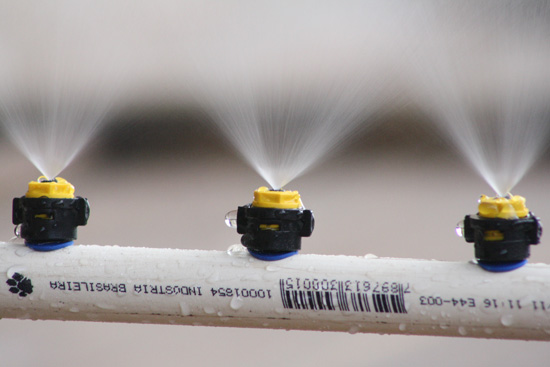
\includegraphics[scale=0.5]{04-figuras/nebulizador.jpg}
\begingroup
\caption{Sistema nebulizador}
\vspace{-\baselineskip}
\fonte{\url{https://www.growshop.com.br/media/wysiwyg/Close_Jato_NA-1_1.jpg}}
\label{fig:nebulizador}
\endgroup
\end{figure}

A nebulização também é utilizada na conservação de flores, estábulos, granjas, balcões de verduras em supermercados, entre outros. O controle do clima ou microclima nas estufas é baseado no princípio da troca de energia entre o ar e a água nebulizada, onde uma caloria representa a quantidade de calor necessária para aumentar em 1 °C a temperatura de 1 cm³ de água.

Em um sistema de nebulização eficiente pode se reduzir de 4 ºC a 6 ºC a temperatura na estufa, em relação às condições externas, ou seja, temperatura e umidade externa. A figura \ref{fig:nebulizador} mostra um sistema nebulizador.

\subsection{Setor de Fruticultura do campus Muzambinho}

No setor de fruticultura do IFSULDEMINAS campus Muzambinho é realizado o cultivo de mudas por estaquia. Esse cultivo é realizado em ambiente de cultivo protegido, como mostra a figura \ref{fig:fruticultura}. Este ambiente conta com um sistema de nebulizador responsável por controlar a temperatura e umidade do ar dentro do ambiente protegido.

O sistema nebulizador existente no setor é controlado por meio de um Arduino que efetua o acionamento de forma programada a cada 10 minutos.

\begin{figure}[H]
    \centering
    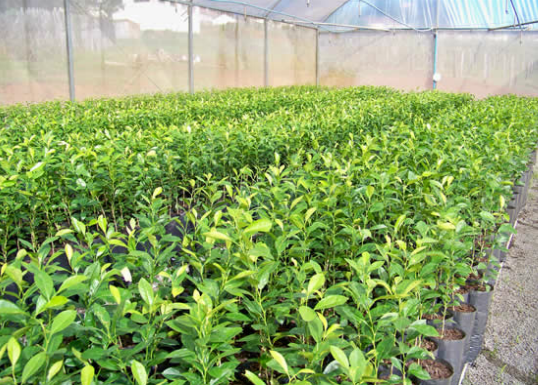
\includegraphics[scale=1]{04-figuras/fruticultura.png}
    \caption{Setor de fruticultura campus Muzambinho}
    \vspace{-\baselineskip}
    \fonte{Setor de Fruticultura do campus Muzambinho}
    \label{fig:fruticultura}
\end{figure}

\section{Internet das Coisas}

A Internet das Coisas (IoT, do inglês Internet of Things) vem se tornando algo comum em sociedade e visa conectar a vida cotidiana a objetos que possuem a internet como meio de comunicação. Essa interconexão de dispositivos na internet possibilita a comunicação dos mesmos com humanos ou até com outros dispositivos conectados \cite{leandro2017}.

\subsection{Rede de Sensores sem Fio}

Nos últimos anos, devido ao avanço tecnológico na área de sensores e comunicação sem fio, houve a criação das Redes de Sensores sem Fio (RSSF). Este tipo de rede pode atuar em diferentes atividades, como monitoramento, rastreamento, entre outras.

As redes de sensores sem fio se diferem das redes convencionais por serem compostas por diversos nos distribuídos além de possuir limitação quanto ao alcance e energia. Cada nó da rede é composto por diversos sensores tais como temperatura, infravermelho, pressão, etc, e esses nós podem ser organizados como \textit{clusters} onde pelo menos um nós seja capaz de detectar algum evento na região e comunicar este evento aos demais nós conectados na rede \cite{loureiro2003redes}.

\citeonline{rocha2007rede}, afirma que essas são algumas características que podem influenciar no projeto de uma rede de sensores sem fio:

\begin{itemize}[itemsep=0em]
    \item Tolerância a falhas: os sensores que compõem os nós são muito pequenos, o que contribui ao fato de eles serem pouco confiáveis, fazendo com que a rede tenha que ser tolerante a falhas. O nível de tolerância de falhas vai depender de cada aplicação. 
    \item Escalabilidade: o fato de os nós serem compostos por equipamentos de baixo custo e tamanho pequeno contribui para a criação de redes de alta escala, necessitando de poucos cuidados e baixo custo de instalação.
    \item Consumo de energia: a energia é um fator crucial em uma rede de sensores sem fio pois as fontes de energia são escassas. Dessa forma os nós devem usar a energia de forma eficiente, ficando "adormecidos" durante os períodos em que não forem necessários.
\end{itemize}

\section{Protocolo MQTT}

\textit{Message Queue Telemetry Transport} (MQTT), este protocolo foi desenvolvido pela IBM no final dos anos 90. 


\section{Microcontrolador}

Microcontroladores são dispositivos eletrônicos que possuem basicamente um microprocessador, memória e interfaces de entrada e saída. Estes dispositivos podem ser programados utilizando alguma linguagem de programação compatível, além de também poder trabalhar com diversos periféricos. Dito de outra forma

\begin{citacao}
	Microcontroladores são computadores de propósito específico. Eles possuem 
tamanho reduzido, baixo custo e baixo consumo de energia. Devido a esses fatores há diversos segmentos, que os utilizam, tais como a indústria automobilística, de telecomunicações, de brinquedos, de eletrodomésticos, de eletroeletrônicos, bélica [\ldots]. \cite{silva2009}  
\end{citacao}

De acordo com \citeonline[p.~15]{martins2005microcontroladores}, exitem diversos tipos de microcontroladores, sendo diferenciados por características como: a velocidade de processamento, a quantidade de memória disponível para armazenar dados e instruções, a quantidade de pinos de entrada e saída, entre outras.

\subsection{ESP8266} 

O modulo ESP8266 é um microcontrolador desenvolvido pela companhia Chinesa Espressif Systems.
O grande diferencial desse microcontrolador é possuir seu próprio sistema de comunicação WIFI, o que o faz ser grandemente utilizado como modulo WIFI por outros microcontroladores, como o Arduino por exemplo, apesar de possuir seu próprio processador, o que torna possível a criação de sistemas embarcados utilizando apenas o ESP8266 \cite[p.~26-27]{kolban2015espbook}.

A tabela \ref{tab:esp8266} mostra as especificações técnicas do ESP8266:

\begin{table}[H]
\centering
\caption{Especificações técnicas do ESP8266}
\begin{tabular}{c|c}
\hline
Voltagem 						& 3.3V 					\\\hline
Consumo de corrente 			& 10uA 					\\\hline
Memória Flash 					& 16MB max				\\\hline
Processador 					& Tensilica L106 32bit	\\\hline
Velocidade do Processador 		& 80-160MHz				\\\hline
RAM 							& 32K + 80K 			\\\hline
GPIOs 							& 17		 			\\\hline
Analógico para digital 			& 1 (1024 de resolução)	\\\hline
Suporte 802.11 					& b/g/n/d/e/i/k/r		\\\hline
Máxima corrente de conexão TCP	& 5						\\\hline
\end{tabular}
\label{tab:esp8266}
\fonte{\cite[p.27]{kolban2015espbook}}
\end{table}


\subsection{ESP-12}

Este módulo possui mais entradas e saídas, o que possibilita a leitura de vários sensores, sendo o ideal para compor um nó da rede de sensores.

\begin{figure}[H]
\centering
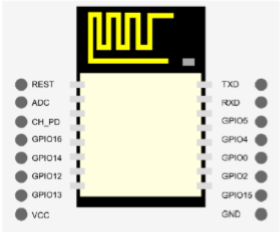
\includegraphics[scale=1]{./04-figuras/esp-12.png}
\begingroup
\caption{GPIOs do ESP-12}
\vspace{-\baselineskip}
\label{fig:esp12-gpios}
\fonte{\cite[p.29]{kolban2015espbook}}
\endgroup
\end{figure}

A figura \ref{fig:esp12-gpios} mostra o posicionamento de cada um dos pinos no ESP-12, as especificações e particularidades de cada um deles é apresentado na tabela \ref{tab:esp12-especificacoes}.

\begin{table}[H]
\centering
\caption{Especificações dos GPIOs}
\label{tab:esp12-especificacoes}
\begin{tabular}{l|l}
\hline
\multicolumn{1}{c|}{\textbf{Nome}} & \multicolumn{1}{c}{\textbf{Descrição}}                                                                                                                     \\ \hline
VCC                                 & 3.3V                                                                                                                                                        \\ \hline
GPIO 13                             & Pode ser usado como SPI MOSI                                                                                                                                \\ \hline
GPIO 12                             & Pode ser usado como SPI MOSI                                                                                                                                \\ \hline
GPIO 14                             & Pode ser usado como SPI MOSI                                                                                                                                \\ \hline
GPIO 16                             &                                                                                                                                                             \\ \hline
CH\_PD                              & \begin{tabular}[c]{@{}l@{}}Enable do ESP8266\\ Nível lógico 1 - Ativado\\ Nível lógico 0 - Desativado\end{tabular}                                          \\ \hline
ADC                                 & Entrada analógico para digital                                                                                                                              \\ \hline
Reset                               & \begin{tabular}[c]{@{}l@{}}1 - Normal\\ 0 - Reset\end{tabular}                                                                                              \\ \hline
TXD                                 & Transmissão serial                                                                                                                                          \\ \hline
RXD                                 & Recepção serial                                                                                                                                             \\ \hline
GPIO 4                              & GPIO normal                                                                                                                                                 \\ \hline
GPIO 5                              & GPIO normal                                                                                                                                                 \\ \hline
GPIO 0                              & \begin{tabular}[c]{@{}l@{}}Deve estar em nível lógico 1 para inicialização do programa (boot mode)\\ e 0 para carregar o programa (flash mode)\end{tabular} \\ \hline
GPIO 2                              & Deve estar em nível lógico 1 para inicialização do programa (boot mode)                                                                                     \\ \hline
GPIO 15                             & \begin{tabular}[c]{@{}l@{}}Deve estar em nível lógico 0 para carregar o programa (flash mode)\\ e para inicialização do programa (boot mode)\end{tabular}   \\ \hline
GND                                 & Terra                                                                                                                                                       \\ \hline
\end{tabular}
\fonte{\cite[p.29]{kolban2015espbook}}
\end{table}

\subsection{Plataforma NodeMCU}

NodeMCU é uma plataforma \textit{Open Source} baseado no microcontrolador ESP8266. Basicamente essa plataforma é composta por um microcontrolador (ESP8266, ESP-12) e uma porta micro USB utilizada para alimentação e programação da placa. Principais características do NodeMCU:
\begin{itemize}[itemsep=0em]
\item Processador ESP8266-12E
\item Arquitetura RISC de 32 bits
\item Processador pode operar em 80MHz ou 160MHz
\item 4Mb de memória flash
\item 64Kb para instruções
\item 96Kb para dados
\item WiFi nativo padrão 802.11b/g/n
\item Opera em modo AP, \textit{Station} ou AP + \textit{Station}
\item Pode ser alimentada com 5VDC através do conector micro USB
\item Possui 11 pinos digitais
\item Possui 1 pino analógico com resolução de 10 bits
\item Pinos digitais, exceto o D0 possuem interrupção, PWM, I2C e one wire
\item Pinos operam em nível lógico de 3.3V
\item Pinos não tolerantes a 5V
\item Possui conversor USB Serial integrado
\item Programável via USB ou WiFi (OTA)
\item Compatível com a IDE do Arduino
\item Compatível com módulos e sensores utilizados no Arduino
\end{itemize}

A figura \ref{fig:nodemcu} apresenta uma breve descrição da composição da placa:

\begin{figure}[H]
\centering
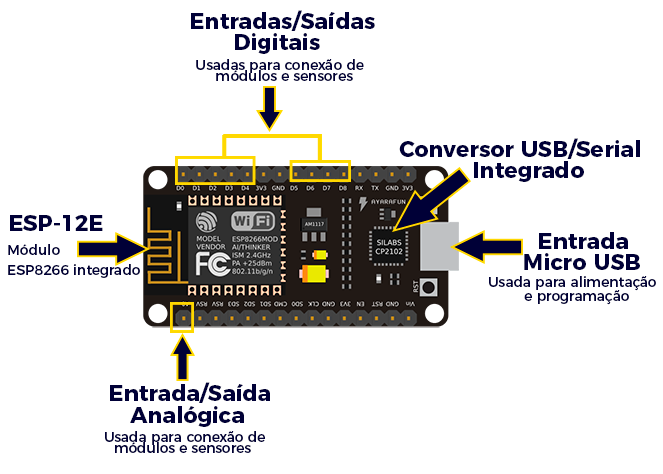
\includegraphics[scale=0.5]{./04-figuras/nodemcu.png}
\caption{Composição do NodeMCU}
\vspace{-\baselineskip}
\fonte{https://goo.gl/VAK2kx}
\label{fig:nodemcu}
\end{figure}

% Falar sobre o Gpio e a programação do nodeMCU

\section{Sensores}

Os sensores são dispositivos que respondem a interações com o ambiente. "Estes dispositivos podem interagir com diversos tipos de grandezas físicas, tais como temperatura, movimento, pressão, entre outras, convertendo essas grandezas em sinais elétricos analógicos ou digitais". \cite{marchesan2012sensores}.

\subsection{Sensor de Temperatura e Umidade do Ar}

O sensor de umidade do ar e temperatura escolhido pra utilização no desenvolvimento do trabalho foi o DHT11, representado na figura \ref{fig:dht11}, que é um sensor comercial de baixo custo. Este sensor utiliza um termistor para medição da temperatura e um sensor capacitivo para medir a umidade do ar \cite{gay2014dht11}.

Características do DHT11:
\begin{itemize}[itemsep=0em]
\item Tensão de alimentação de 3V a 5V
\item Tensão de alimentação máxima 5,5V
\item Corrente de operação 200uA a 500mA
\item Corrente de Stand-By 100uA a 150uA
\item Faixa de medição de umidade 0\% a 90\% com precisão de 5\%
 pra mais ou pra menos
\item Faixa de medição de temperatura 0ºC a 50ºC com precisão de 2\% pra mais ou para menos
\item Tempo de resposta <5s
\item Dimensões 23 x 12 x 5mm (incluindo os terminais)
\end{itemize}

\begin{figure}[H]
\centering
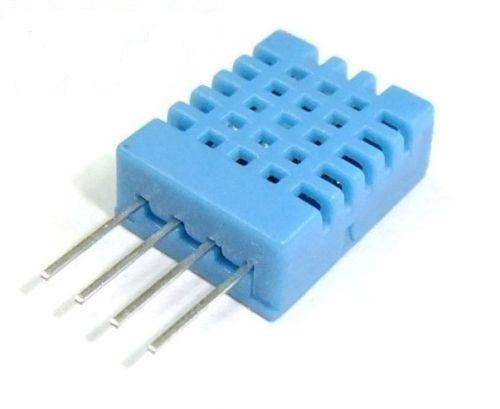
\includegraphics[scale=0.3]{./04-figuras/sensor_DHT11.jpg}
\caption{Sensor de umidade e temperatura}
\vspace{-\baselineskip}
\fonte{Do autor}
\label{fig:dht11}
\end{figure}


\subsection{Sensor de Molhamento Foliar}

Os sensores do tipo resistivo são comumente empregados para medição da duração do molhamento foliar, quando há água em sua superfície a resistência elétrica é reduzida devido a um curto-circuito proveniente da presença do líquido. Estes tipos de sensores são capazes apenas de detectar se há ou não água sobre a sua superfície, se precisarmos quantificar esse liquido será necessário a utilização de um sensor do tipo capacitivo.

Os sensores do tipo capacitivo trabalham da seguinte maneira:
\begin{itemize}[itemsep=0em]
\item quando não há a presença de nenhum liquido, o seu dielétrico é apenas o ar
\item conforme sua superfície entra em contato com algum líquido, parte do seu dielétrico se torna a água, que possui permissividade aproximadamente 80 vezes maior do que a do ar, provocando assim um aumento na capacitância. 
\end{itemize}
Dessa forma, ao medirmos a capacitância do sensor, poderemos estimar a quantidade de água que se encontra em sua superfície.
A figura \ref{fig:molhamento} mostra o sensor de molhamento foliar utilizado no trabalho.

\begin{figure}[H]
\centering
\setlength\lineskip{0pt}
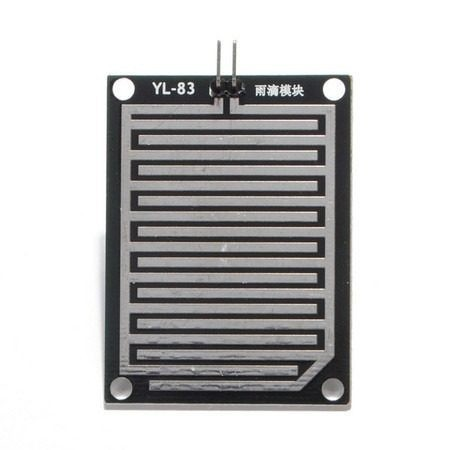
\includegraphics[scale=0.3]{./04-figuras/molhamento.jpg}
\caption{Sensor de Molhamento Foliar}
\vspace{-\baselineskip}
\fonte{Do autor}
\label{fig:molhamento}
\end{figure}

\begin{comment}
\subsection{Sensor de Luminosidade}

\textit{Light Dependant Resistor} (LDR) como mostra a figura \ref{fig:ldr} é um resistor cuja sua resistência varia de forma inversamente proporcional a incidência de luz, ou seja, quanto maior a iluminação menor será o valor da resistência \cite[p.114]{mcroberts2011arduinobasico}.

\begin{figure}[H]
\centering
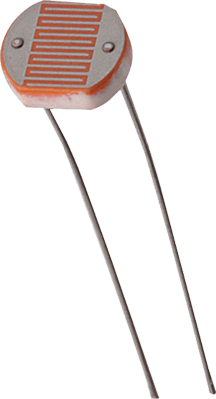
\includegraphics[scale=0.3]{./04-figuras/ldr.png}
\caption{Sensor de luminosidade (LDR)}
\vspace{-\baselineskip}
\fonte{Do autor}
\label{fig:ldr}
\end{figure}

Na tabela \ref{tab:vout-ldr} podemos constatar a variação dos valores de tensão de saída (Vout), indo de mais escuro para mais claro, para um LDR com tensão de entrada (Vin) de 5V e resistência de 10k$\Omega$ como divisor de tensão.

\begin{table}[H]
\centering
\caption{Valores de Vout (voltagem de saída) para um LDR com 5V como Vin (voltagem de entrada)}
\begin{tabular}{c|c|c|c}
\hline
\textbf{R1} & \textbf{R2 (LDR)} & \textbf{Vout} & \textbf{Claridade} 	\\\hline
10k$\Omega$ & 100k$\Omega$ 		& 4,54V 		& Mais escuro			\\\hline
10k$\Omega$ &  73k$\Omega$ 		& 4,39V 		& 25\%					\\\hline
10k$\Omega$ &  45k$\Omega$ 		& 4,09V 		& 50\%    				\\\hline
10k$\Omega$ &  28k$\Omega$ 		& 3,68V 		& 75\%    				\\\hline
10k$\Omega$ &  10k$\Omega$ 		& 2,50V 		& Mais claro    		\\\hline
\end{tabular}
\fonte{\citeonline[p.~119]{mcroberts2011arduinobasico}}
\label{tab:vout-ldr}
\end{table}
\end{comment}

\section{Atuadores}

Os atuadores são componentes que convertem energia, seja ela elétrica, hidráulica ou pneumática, em grandeza física, como movimento, calor, etc. Além disso os atuadores "atendem a comandos que podem ser manuais ou automáticos, ou seja, qualquer elemento que realize um comando recebido de outro dispositivo, com base em uma entrada ou critério a ser seguido". \cite{brugnari2010automaccao}

\subsection{Relé}

Relé é uma chave eletrônica que liga ou desliga quando recebe uma tensão em seus pinos de controle. Esta chave trabalha de forma diferente das convencionais pois não depende da intervenção humana para o seu acionamento \cite[p.28]{ribeiro1999automaccao}.

A figura \ref{fig:rele} representa a estrutura interna de um relé:

\begin{figure}[H]
\centering
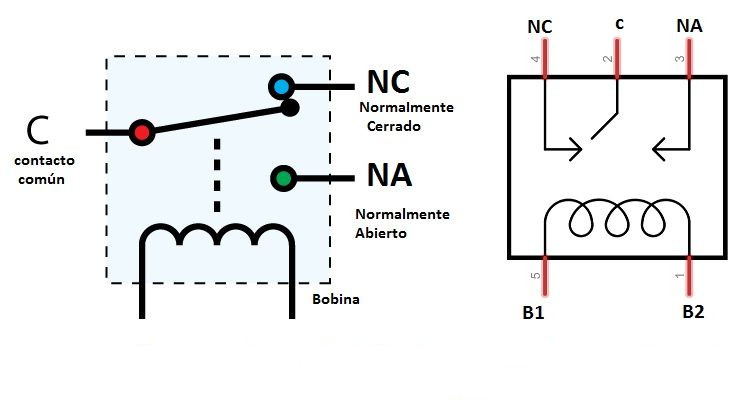
\includegraphics[scale=0.3]{./04-figuras/reles.jpg}
\caption{Estrutura interna do rele}
\vspace{-\baselineskip}
\fonte{http://www.areatecnologia.com/electricidadrele.html}
\label{fig:rele}
\end{figure}

\begin{itemize}[itemsep=0em]
\item B1 e B2 que são os terminais de controle, estes terminais são conectados à uma bobina que quando energizada fecha contato permitindo a passagem de corrente do pino C para o pino NO.
\item \textit{Normally Open} (NO) - normalmente aberto: quando o relé é acionado permite-se passagem de corrente do pino C para o NO.
\item \textit{Normally Close} (NC) - normalmente fechado: quando o relé é acionado passagem de corrente do pino C para o NC é interrompida.
\item \textit{Common Connection} (C) - conexão comum: terminal que é  conectado à fonte externa quando. Normalmente conectado ao pino NC, quando o rele é acionado a conexão é trocada para o pino NO.
\end{itemize}

\begin{figure}[H]
\centering
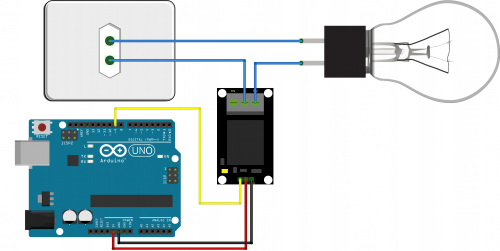
\includegraphics[scale=0.5]{./04-figuras/rele-exemplo.png}
\caption{Exemplo de ligação do rele com o Arduino}
\vspace{-\baselineskip}
\fonte{https://www.robocore.net/tutoriais/modulo-rele-arduino.html}
\label{fig:releligacao}
\end{figure}

A figura \ref{fig:releligacao} nos mostra um exemplo de ligação de um rele à plataforma Arduino, este rele está sendo utilizado para acionar uma lâmpada. Como podemos ver, esta lâmpada está conectada a uma fonte de energia externa, o papel do rele é trabalhar como uma chave que, ao receber uma tensão enviada pelo Arduino, permite a passagem da corrente, que vem da fonte externa, para a lâmpada.
    \chapter{Metodologia}

% \section{Tipo de Pesquisa}
Uma pesquisa científica pode ser classificada quanto à sua abordagem, sua natureza, seus objetivos e seus procedimentos \cite{gerhardt2009tiposdepesquisa}, dessa forma podemos definir que esta pesquisa terá uma abordagem quantitativa, natureza aplicada, objetivo exploratório, e os procedimentos serão de uma pesquisa exploratória.

Esta seção apresenta a metodologia que será empregada no desenvolvimento do trabalho proposto, visando alcançar os objetivos descritos anteriormente.

% \section{Materiais e Métodos}

\section{Rede de Sensores sem Fio}
A rede de sensores proposta coleta dados de temperatura, umidade do ar e molhamento foliar, com o objetivo de, a partir dos dados coletados, efetuar o controle do sistema nebulizador.

Cada nó da rede é composto por um controlador, neste trabalho foi utilizado a plataforma NodeMCU. Este controlador esta conectado aos sensores DHT11 (responsável pela coleta de temperatura e umidade) e o sensor de molhamento foliar. Todos os nós estão conectados à internet por meio de uma rede \textit{wifi}. A figura \ref{fig:esquema-rede} representa, de forma simples, como é a estrutura da rede.

\begin{figure}[H]
\centering
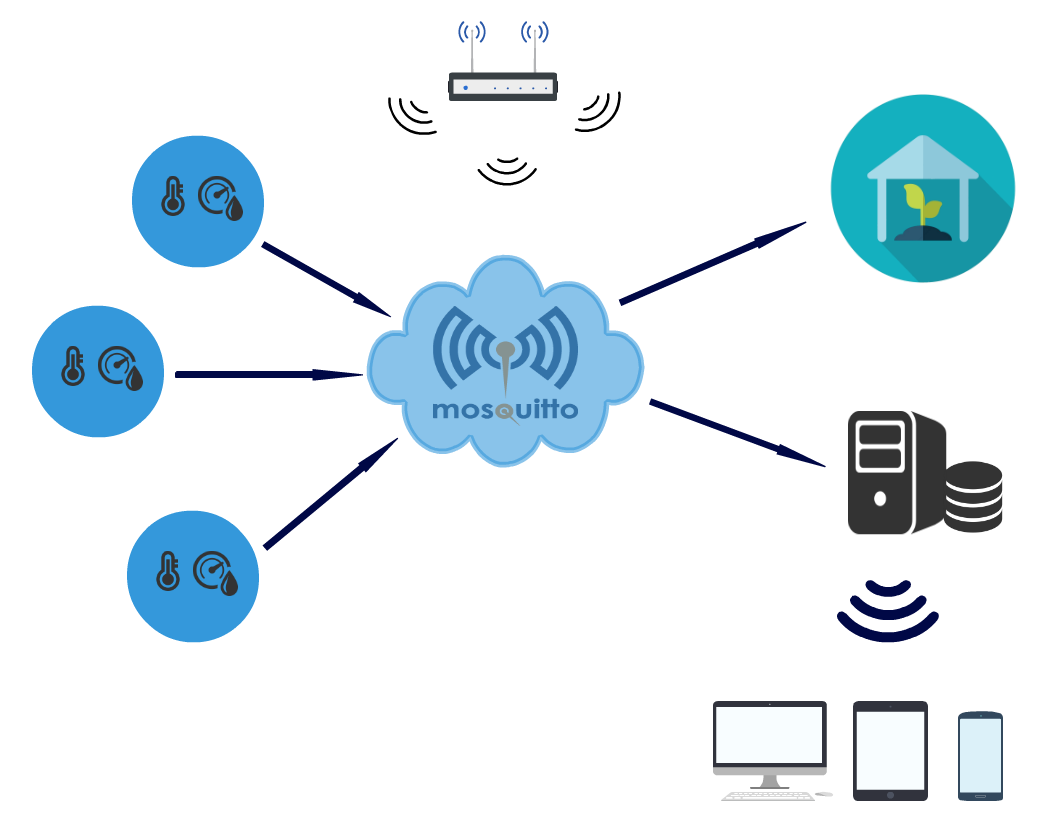
\includegraphics[scale=0.3]{./04-figuras/rede.png}
\caption{Esquema da rede de sensores}
\vspace{-\baselineskip}
\fonte{Do autor}
\label{fig:esquema-rede}
\end{figure}

A comunicação da rede se dá por meio do protocolo MQTT utilizando a ferramenta Mosquitto, que é um \textit{broker} mqtt \textit{open source}. A troca de mensagens da rede segue o seguinte formato:

\begin{table}[H]
\centering
\caption{Formato de das Mensagens trocadas pela rede}
\vspace{-\baselineskip}
\begin{minted}[
frame=single,
framesep=2mm,
baselinestretch=1.2,
bgcolor=LightGray,
fontsize=\footnotesize,
]{js}
{
    "node": {
        "mac": "",          // Endereço MAC do nó
        "ip": "",           // Endereço IP do nó
        "location": "",     // Localização do nó
        "battery": ""       // Nível de bateria do nó
    },
    "sensors": {
        "temperature": "",  // Temperatura
        "humidity": "",     // Umidade do ar 
        "luminosity": "",   // Luminosidade 
        "leafWetness": ""   // Molhamento foliar
    },
    "timestamp": ""         // Data e hora em que a mensagem foi enviada
}
\end{minted}
\label{tab:formato-mensagens}
\vspace{-1.2cm}
\fonte{Do autor}
\end{table}

Há um nó da rede e um cliente web que estão conectados como assinantes da rede, ou seja, estão escutando todas as mensagens que são publicadas. O nó assinante é responsável por coletar os dados publicados e, a partir deles, tomar decisões quanto ao acionamento do sistema nebulizador. Enquanto, o cliente web é responsável por coletar estes dados e armazena-los em um banco de dados, para que os mesmos possam ser exibidos posteriormente ao usuário por meio de relatórios.

% \begin{figure}[H]
% \centering
% 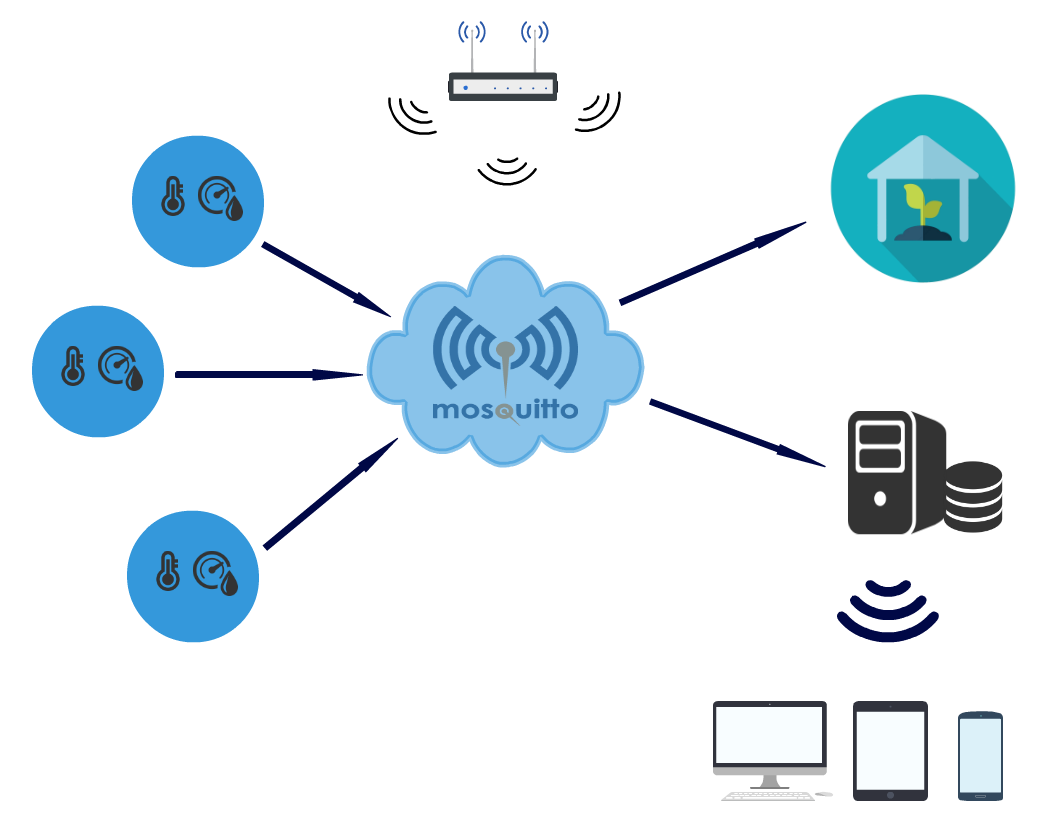
\includegraphics[scale=0.3]{./04-figuras/rede.png}
% \caption{Esquema da rede de sensores}
% \vspace{-\baselineskip}
% \fonte{Do autor}
% \label{fig:esquema-rede}
% \end{figure}

\section{Aplicação Web}
Nesta seção serão apresentados os passos seguidos no desenvolvimento da aplicação, tais como o processo de desenvolvimento de software e tecnologias empregadas.

\subsection{Processo de Desenvolvimento de \textit{Software}} 
O processo de desenvolvimento de \textit{software} utilizado foi o Iterativo e Incremental. Esse processo consiste em um ciclo onde são realizadas tentativas sucessivas de refinamento, a cada iteração são realizadas melhorias no \textit{software}.

\citeonline{bezerra2017iterativoeincremental} define o processo Iterativo e Incremental como um conjunto de ciclos, onde cada ciclo considera um subconjunto de requisitos. Uma vez que estes requisitos são implementados um novo ciclo se inicia, e com este novo ciclo um novo subconjunto de requisitos é considerado para ser desenvolvido, o que produz um novo incremento do sistema. Dessa forma, o desenvolvimento evolui em versões, ao longo da construção incremental e iterativa de novas funcionalidades até que o sistema completo esteja construído.

\begin{figure}[H]
    \centering
    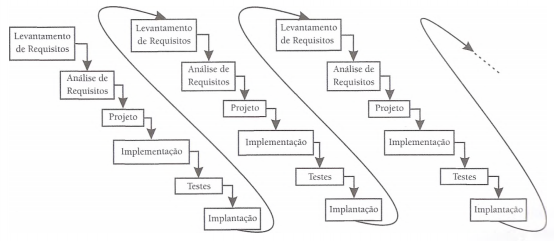
\includegraphics[scale=0.7]{04-figuras/iterativo-incremental.png}
    \caption{Etapas a serem realizadas a cada ciclo}
    \vspace{-\baselineskip}
    \fonte{\cite{bezerra2017iterativoeincremental}}
    \label{fig:iterativo-incremental}
\end{figure}

Como pode ser observado na figura \ref{fig:iterativo-incremental}, cada ciclo do processo Iterativo e Incremental é composto pelas etapas de análise e levantamento de requisitos, projeto de software, implementação, testes e implantação. \citeonline{bezerra2017iterativoeincremental} ainda afirma que a abordagem incremental estimula a participação do usuário nas etapas do desenvolvimento, o que diminui a chance de ocorrer interpretações erradas em relação aos requisitos levantados, além de também possibilitar um melhor gerenciamento em relação aos riscos do projeto.

\subsection{Levantamento e Análise de Requisitos}
O primeiro passo realizado no desenvolvimento do sistema foi o levantamento de requisitos. Este levantamento foi realizado através de reuniões juntamente ao professor responsável pelo setor de fruticultura. Durante estas reuniões foram definidas as funcionalidades que atendem às necessidades do setor. Após o levantamento ser concluído, foi feito uma análise desses requisitos juntamente ao professor orientador do trabalho, onde foi definido um escopo viável para implementar. 

\subsection{Projeto de \textit{Software}}
Para o projeto de \textit{software} foi utilizada a Linguagem de Modelagem Unificada (UML), esta linguagem permite a modelagem de sistemas através de elementos gráficos, como diagramas \cite{bezerra2017iterativoeincremental}. 

\begin{figure}[H]
    \centering
    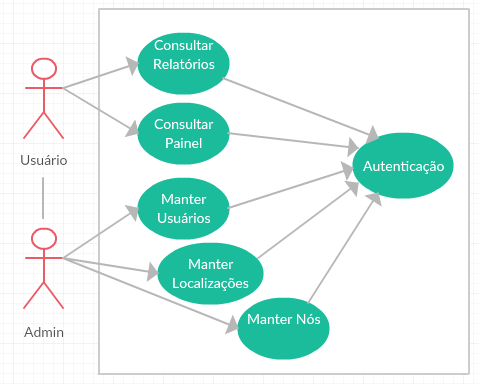
\includegraphics[scale=0.8]{04-figuras/caso_de_uso.png}
    \caption{Diagrama de caso de uso}
    \vspace{-\baselineskip}
    \fonte{Do autor}
    \label{fig:caso-de-uso}
\end{figure}

Nesta etapa foi desenvolvido o diagrama de caso de uso (figura \ref{fig:caso-de-uso}), este diagrama representa a iteração do ator (usuário) com as funcionalidades do sistema através de fluxos \cite{gomes2003casodeuso}.

Como mostra a figura \ref{fig:caso-de-uso}, o sistema conta com dois atores, que representam os
dois grupos de usuários que utilizaram o sistema. O ator "Usuário" tem acesso às funcionalidades de "Consultar Painel" e "Consultar Relatórios", já o ator "Admin", além de herdar estas funcionalidades do ator "Usuário", também possui acesso às funcionalidades de "Manter Localizações", "Manter nós" e "Manter Usuários". Todas as funcionalidades do sistema exigem que o usuário esteja autenticado. O verbo "manter", presente nas funcionalidades, representa quatro operações básicas de banco de dados, \textit{Create, Read, Update e Delete} (CRUD).

\subsection{Implementação}
A implementação do sistema foi dividida em duas partes, \textit{back-end} e \textit{front-end}. O \textit{back-end}, como o próprio nome sugere, é a parte de "trás" da aplicação. É a parte da aplicação que roda no servidor e é responsável pela implementação da regra de negócio. Já o termo \textit{front-end} se refere à parte de interface do sistema, ou seja, é a parte da aplicação que interage diretamente com o usuário.

\subsubsection{\textit{Back-end}}
O \textit{backend} foi desenvolvido utilizando NodeJS\footnote{Mais informações sobre Nodejs podem ser acessadas em: \url{https://nodejs.org/en/}}, que é um interpretador JavaScript \textit{open source} que possibilita a sua utilização como linguagem de servidor, através do \textit{framework web} AdonisJS\footnote{Mais informações sobre Adonisjs podem ser acessadas em: \url{https://adonisjs.com/}}. O desenvolvimento seguirá o padrão \textit{Model, View, Controller} (MVC).

\begin{figure}[H]
    \centering
    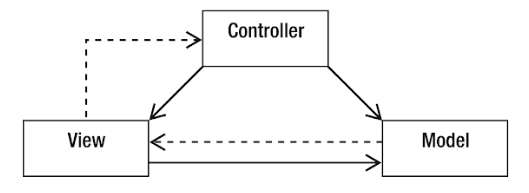
\includegraphics[scale=1]{04-figuras/mvc.png}
    \caption{Arquitetura do padrão MVC}
    \vspace{-\baselineskip}
    \fonte{\cite{dooley2011mvc}}
    \label{fig:mvc}
\end{figure}

Como podemos ver na figura \ref{fig:mvc}, o padrão MVC se divide em três camadas:
\begin{itemize}[itemsep=0em]
    \item \textit{\textbf{Controller}} (controlador): o controlador interpreta as entradas enviadas pelo usuário e as mapeia em comandos que serão enviados para o modelo e/ou para uma janela de visualização \cite{dooley2011mvc}.
    \item \textit{\textbf{Model}} (modelo): o modelo gerencia os elementos de dados, nesta camada que é realizado a comunicação com o banco de dados  \cite{dooley2011mvc}.
    \item \textit{\textbf{View}} (visão): visão é a camada responsável por apresentar os dados ao usuário \cite{dooley2011mvc}.
\end{itemize}

Como banco de dados foi escolhido o MongoDB, que é um software de banco de dados \textit{open source} orientado a documentos e multiplataforma. 
\vfill

\subsubsection{\textit{Front-end}}
O \textit{front-end} do sistema foi desenvolvido utilizando a linguagem JavaScript por meio da biblioteca ReactJS. Esta biblioteca foi desenvolvida pela equipe de desenvolvedores do Facebook e Instagram, é uma biblioteca que funciona na ideia de componentização, onde a ideia é quebrar os elementos em pequenos componentes reutilizáveis. Para desenvolvimento da interface foram empregados os conceitos de \textit{Material Design} por meio do \textit{framework} Material UI que implementa esse conceito.

\subsection{Testes e Implantação}
Nesta etapa do desenvolvimento serão realizados testes automatizados nas funcionalidades do sistema. Após testadas as funcionalidades serão efetuados testes de usabilidade da aplicação buscando um \textit{feedback} do usuário para que o sistema possa ser melhorado. Realizado os devidos testes se dará inicio a mais um ciclo de desenvolvimento, este ciclo se repetirá até que o sistema completo esteja concluído e valido para que possa ser implantado.

\section{Experimentos}
Nesta etapa serão efetuados experimentos visando verificar se o trabalho desenvolvido cumpre a proposta de trazer melhorias na produção. Serão separados dois ambientes distintos:

\begin{itemize}[itemsep=0em]
\item O primeiro ambiente estará sob as condições atuais onde o sistema nebulizador é acionado de maneira estática.
\item O segundo ambiente estará sendo controlado pelo sistema desenvolvido.
\end{itemize}

Serão colocadas mudas nos dois ambientes para que possa ser avaliado sob quais condições será obtido o melhor resultado.
    \chapter{Resultados e Discussão}

\section{Rede de Sensores Sem Fio}
Nesta seção serão apresentados os resultados parciais obtidos no desenvolvimento da Rede de Sensores sem fio.

\subsection{Testes utilizando a IDE Arduino}
Inicialmente foram efetuados testes utilizando o módulo NodeMCU sendo programado utilizando-se a IDE do Arduino. Para efetuar a leitura do sensor de temperatura e umidade do ar de uma forma mais simples foi utilizado a biblioteca DHT.h. Como resultado foram obtidos alguns códigos, apresentados nos Quadros \ref{tab:funcao-temperatura}, \ref{tab:funcao-umidade} e \ref{tab:funcao-request}:

\begin{quadro}[H]
\centering
\caption{Função que lê a temperatura do sensor.}
\vspace{-\baselineskip}
\begin{minted}[
frame=single,
framesep=2mm,
baselinestretch=1.2,
bgcolor=LightGray,
fontsize=\footnotesize,
% linenos
]{c++}

float getTemperature() {
    float temp = dht.readTemperature();
    
    if (isnan(temp)) {
        Serial.println("Failed to read from DHT sensor!");
        return;
    }
    
    return temp;
}
\end{minted}
\vspace{-1.2cm}
\label{tab:funcao-temperatura}
\fonte{Do Autor (2018).}
\end{quadro}

O Quadro \ref{tab:funcao-temperatura} mostra uma função que é responsável por efetuar a coleta de temperatura pelo sensor DHT11, essa temperatura pode ser coletada em Celsius ou em Fahrenheit, neste caso iremos utilizar apenas o valor em celsius.

\begin{quadro}[H]
\centering
\caption{Função que lê a umidade do sensor.}
\vspace{-\baselineskip}
\begin{minted}[
frame=single,
framesep=2mm,
baselinestretch=1.2,
bgcolor=LightGray,
fontsize=\footnotesize,
% linenos
]{c++}

float getHumidity() {
    float hum = dht.readHumidity();
    
    if (isnan(hum)) {
        Serial.println("Failed to read from DHT sensor!");
        return;
    }
    
    return hum;
}
\end{minted}
\vspace{-1.2cm}
\label{tab:funcao-umidade}
\fonte{Do Autor (2018).}
\end{quadro}

Já no Quadro \ref{tab:funcao-umidade} temos o a função que é responsável por efetuar a coleta de umidade do ar pelo sensor DHT11. O valor é coletado em porcentagem.

\begin{quadro}[H]
\centering
\caption{Função que envia um objeto JSON com os valores medidos.}
\vspace{-\baselineskip}
\begin{minted}[
frame=single,
framesep=2mm,
baselinestretch=1.2,
bgcolor=LightGray,
fontsize=\footnotesize,
% linenos
]{c++}

void sendRequest(WiFiClient client) {
  StaticJsonBuffer<400> jsonBuffer;

  JsonObject& data = jsonBuffer.createObject();

  data["humidity"] = getHumidity();
  data["temperature"] = getTemperature();

  client.println(String("POST ") + url + " HTTP/1.1");
  client.println(String("Host: ") + host);
  client.println("Cache-Control: no-cache");
  client.println("Content-Type: application/json");
  client.print("Content-Length: ");
  client.println(data.measurePrettyLength());

  client.println();

  data.prettyPrintTo(client);
}
\end{minted}
\vspace{-1.2cm}
\label{tab:funcao-request}
\fonte{Do Autor (2018).}
\end{quadro}

Esta função (Quadro \ref{tab:funcao-request}) monta um objeto JSON contendo os valores obtidos pelo sensor de temperatura e umidade do ar DHT11. Após montar este objeto é feito uma requisição do tipo POST na aplicação Web onde será armazenado em um banco de dados.

\subsection{Desenvolvimento utilizando MicroPython}

Depois de realizados estes testes utilizando a IDE do Arduino, foi instalado o \textit{firmware} MicroPython que possibilita que o módulo NodeMCU seja programado utilizando-se a linguagem de Programação Python.

A programação foi realizada da seguinte forma, o nó se conecta a uma rede \textit{wifi} (Quadro \ref{tab:funcao-conecta}) e, após estar conectado, faz a coleta de dados de todos os sensores ligados a ele (Quadro \ref{tab:funcao-coleta}). Após coletar os dados, eles são publicados no broker mqtt (Quadro \ref{tab:funcao-publica}), feito isso, o nó entra em modo \textit{sleep}. Este ciclo irá se repetir constantemente, sendo que o nó será acordado apos um intervalo de tempo pré definido.

\begin{quadro}[H]
\centering
\caption{Função que conecta o nó a uma rede wifi.}
\vspace{-\baselineskip}
\begin{minted}[
frame=single,
framesep=2mm,
baselinestretch=1.2,
bgcolor=LightGray,
fontsize=\footnotesize,
% linenos
]{python}

def do_connect():
    networks = list(wifi.scan())
    for net in networks:
        if (net[0].startswith('AP_IFSUL') 
            or net[0].startswith('IF-CampusMuz')) 
            and net[4] == 0:
            
            wifi.connect(str(net[0].decode()), '')

            for t in range(0, 120):
                if wifi.isconnected():
                    return True

                time.sleep_ms(400)

            return None

\end{minted}
\vspace{-1.2cm}
\label{tab:funcao-conecta}
\fonte{Do Autor (2018).}
\end{quadro}

\begin{quadro}[H]
\centering
\caption{Função que coleta os dados dos sensores.}
\vspace{-\baselineskip}
\begin{minted}[
frame=single,
framesep=2mm,
baselinestretch=1.2,
bgcolor=LightGray,
fontsize=\footnotesize,
% linenos
]{python}

def get_sensors_data(self):

    dhtSensor = DHTSensor(
        vcc=self.conf['dht']['vcc'], 
        signal=self.conf['dht']['signal']
    )
    
    leafWetnessSensor = LeafWetnessSensor(
        vcc=self.conf['leafWetness']['vcc'],
        signal=self.conf['leafWetness']['signal']
    )
        
    tick = time.ticks_ms()
    while True:
        delta = time.ticks_diff(time.ticks_ms(), tick)
        if delta > (200):
            break

    dhtValues = dhtSensor.get_value()
    leafWetnessValue = leafWetnessSensor.get_value()

    data = {
        'humidity': dhtValues['humidity'],
        'temperature': dhtValues['temperature'],
        'leafWetness': leafWetnessValue
    }

    dhtSensor.__del__()
    leafWetnessSensor.__del__()

\end{minted}
\vspace{-1.2cm}
\label{tab:funcao-coleta}
\fonte{Do Autor (2018).}
\end{quadro}

\begin{quadro}[H]
\centering
\caption{Função que publica os dados.}
\vspace{-\baselineskip}
\begin{minted}[
frame=single,
framesep=2mm,
baselinestretch=1.2,
bgcolor=LightGray,
fontsize=\footnotesize,
% linenos
]{python}

def send_data(self):
    id = 'esp8266_' + ubinascii.hexlify(machine.unique_id()).decode()
    HOST = self.conf['mqtt']['host']
    PORT = self.conf['mqtt']['port']
    USER = self.conf['mqtt']['user']
    PASS = self.conf['mqtt']['pass']
    topic = self.conf['mqtt']['topic']

    node = self.get_node_information()
    sensors = self.get_sensors_data()

    data = { 'node': node, 'sensors': sensors }

    mqtt_client = MQTTClient(id, HOST, PORT, USER, PASS)
    
    try:
        mqtt_client.connect()

        mqtt_client.publish(topic, json.dumps(data))

        while True:
            data = self.get_saved_data()

            if data is not None:
                mqtt_client.publish(topic, json.dumps(data))
            else:
                break
        
        mqtt_client.disconnect()

    except:            
        if not self.save_data(data):
            machine.reset()

\end{minted}
\vspace{-1.2cm}
\label{tab:funcao-publica}
\fonte{Do Autor (2018).}
\end{quadro}

\subsection{Montagem dos Nós}
A montagem dos nós foi feita utilizando \textit{protoboard}, que são placas para experimentação onde não é necessário soldar os componentes do circuito. Os componentes foram conectados seguindo o esquema mostrado na Figura \ref{fig:no-publicador}.

Na Figura \ref{fig:no-interno}, podemos ver os componentes dispostos dentro de uma caixa de pvc impermeável, onde eles serão encapsulados. A caixa foi vedada com silicone para evitar que os componentes tenham contato com a água que aspergida pelo sistema de nebulização. 

\begin{figure}[H]
    \centering
    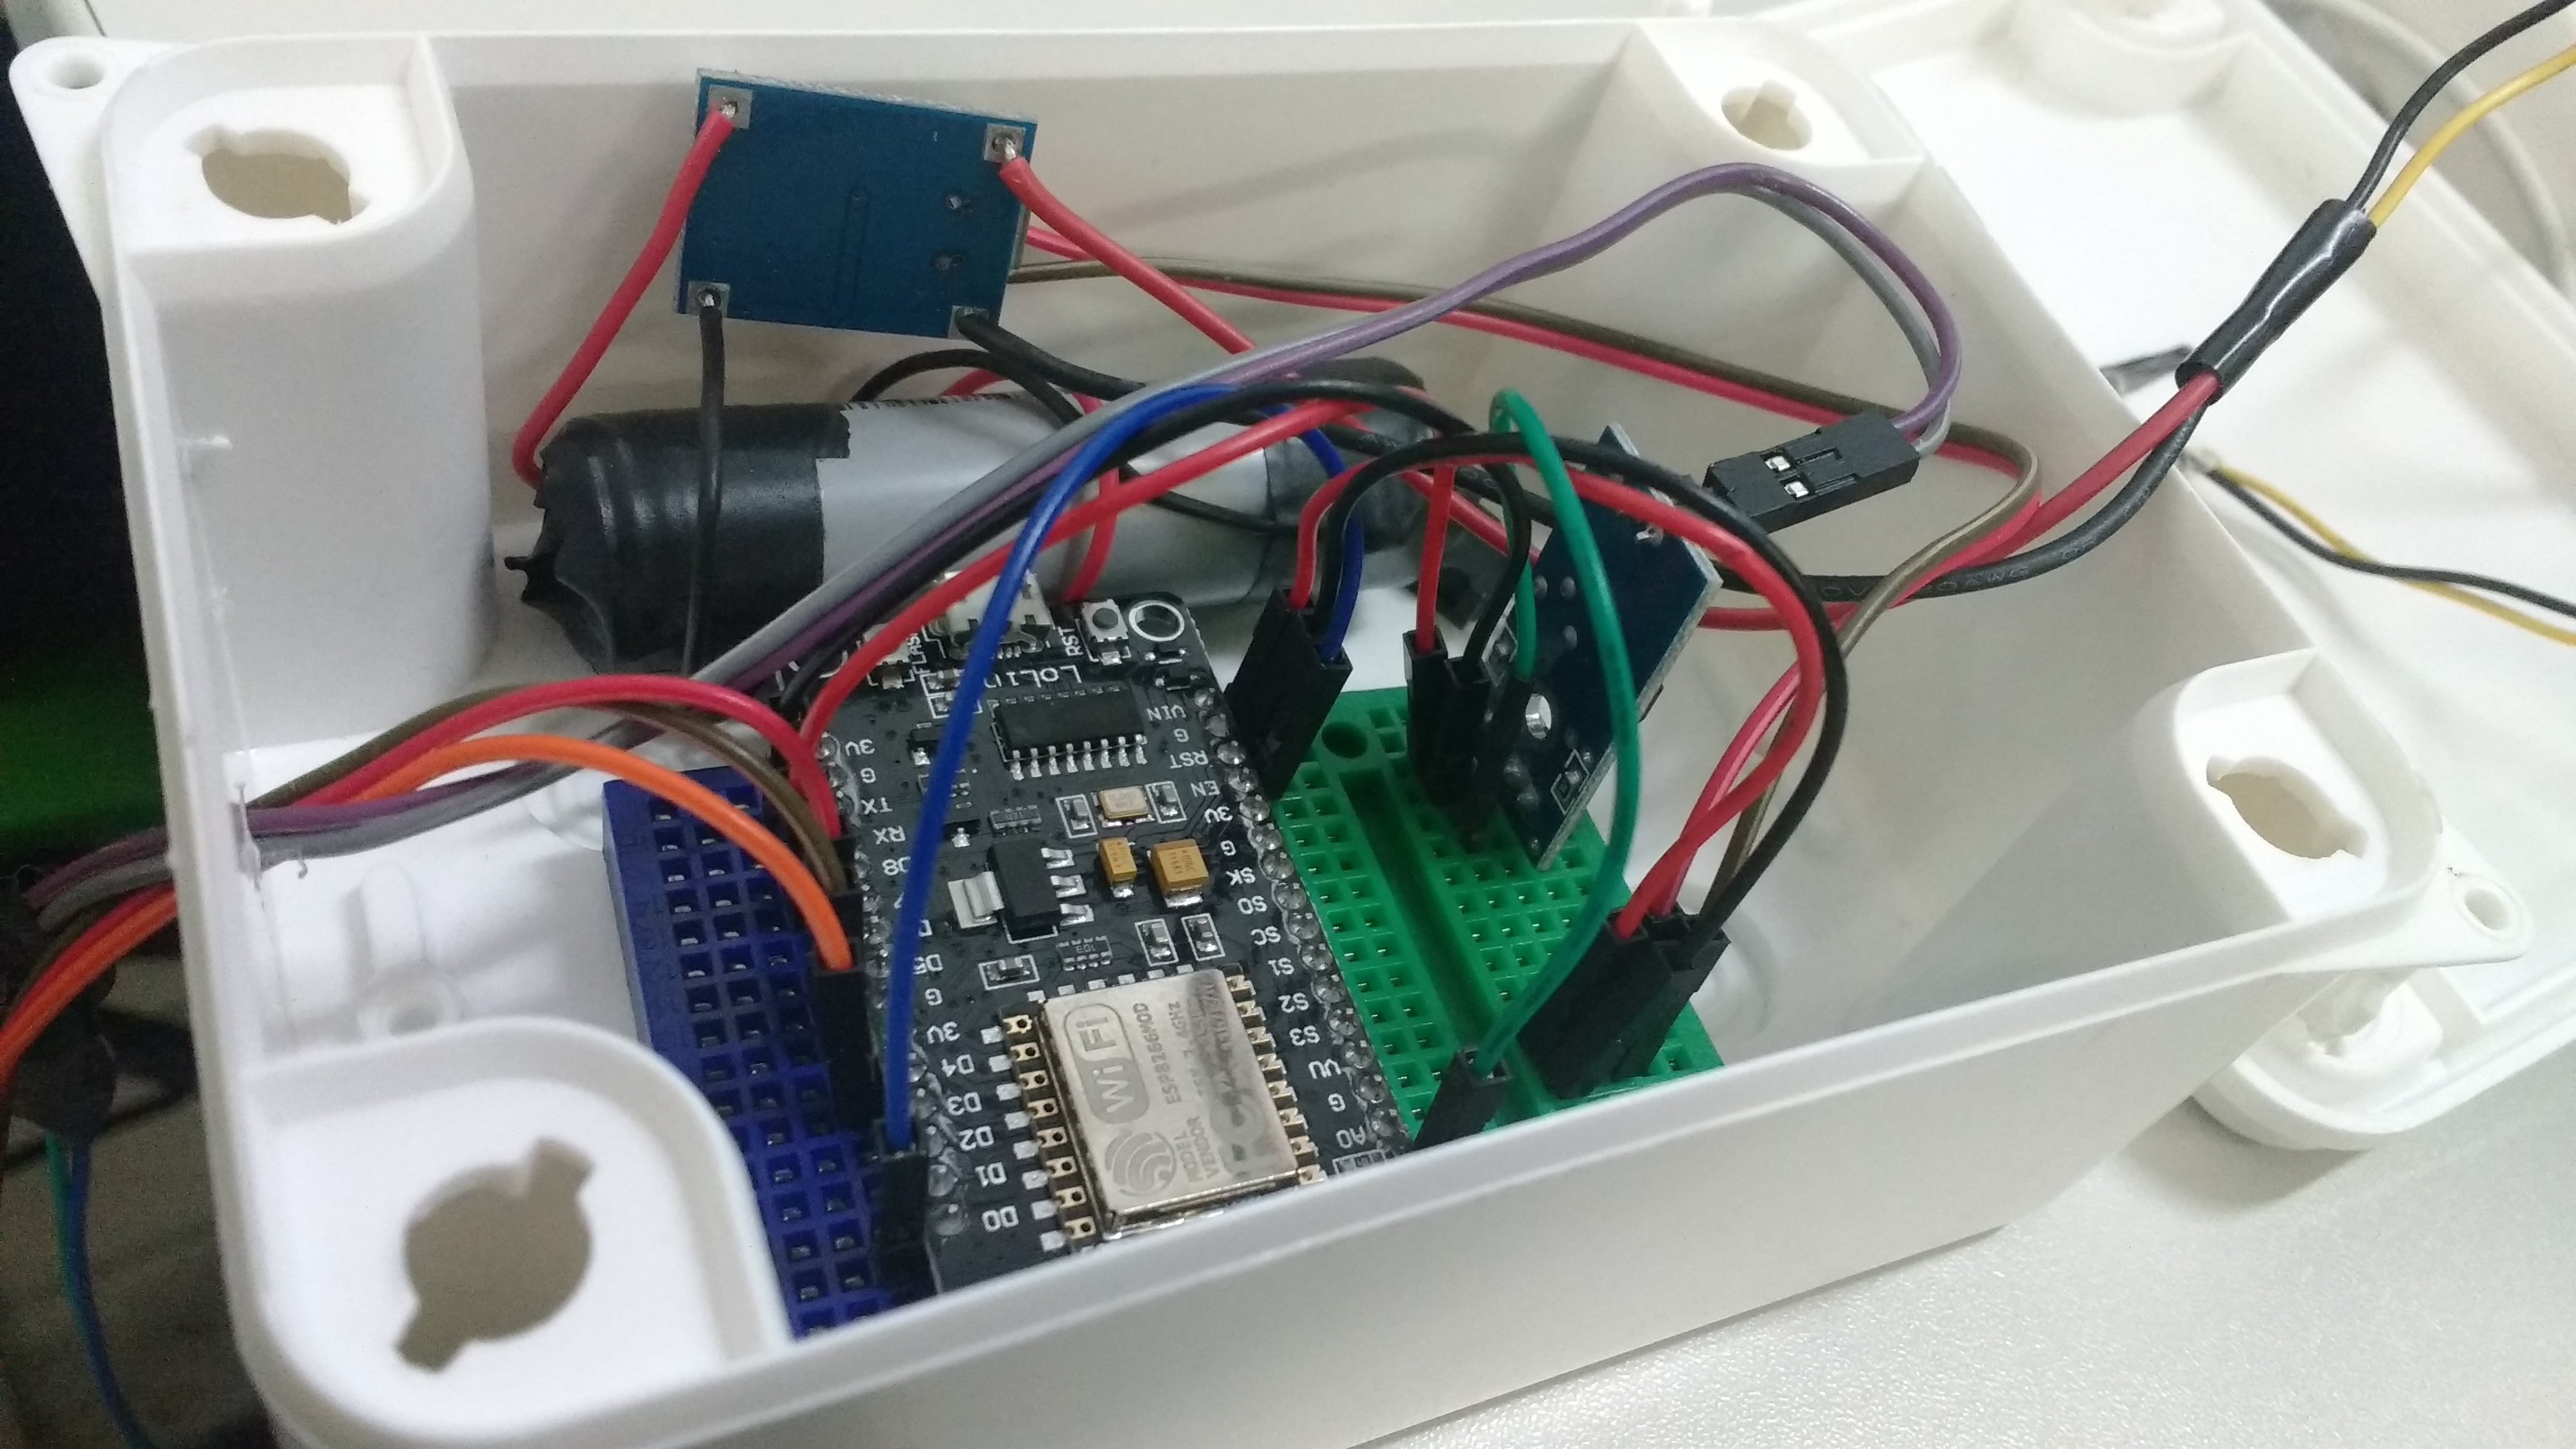
\includegraphics[scale=0.1]{04-figuras/no-interior.jpg}
    \caption{Parte interna de um nó publicador.}
    \vspace{-\baselineskip}
    \fonte{Do Autor (2018).}
    \label{fig:no-interno}
\end{figure}

Já na Figura \ref{fig:no-externo2} temos o nó já encapsulado, podemos ver o painel solar que foi posicionado no topo da caixa e os sensores de umidade relativa do ar, temperatura e molhamento foliar que estão ligados ao controlador por meio de fios.

\begin{figure}[H]
    \centering
    \includegraphics[scale=0.13]{04-figuras/no-exterior2.png}
    \caption{Nó encapsulado pronto para ser instalado.}
    \vspace{-\baselineskip}
    \fonte{Do Autor (2018).}
    \label{fig:no-externo2}
\end{figure}

\section{Aplicação Web}
Nesta seção serão apresentados os resultados parciais obtidos quanto ao desenvolvimento da aplicação web, seguindo os passos listados na Metodologia, seção 4.

\subsection{Levantamento e Análise de Requisitos}
Foram levantados os requisitos que atendem às necessidades do setor. Feito este levantamento, foi definido um escopo para se dar inicio ao desenvolvimento, foi definido que as funcionalidades a serem implementadas serão: 

\begin{itemize}[itemsep=0em]
\item Manter usuários
\item Manter experimentos
\item Manter medições
\item Consultar relatórios
\end{itemize}

\subsection{Projeto de \textit{software}}
A figura \ref{fig:caso-de-uso} mostra o diagrama de caso de uso elaborados de acordo com os requisitos levantados na etapa anterior.

\subsection{Implementação e Implantação}
A figura \ref{fig:tela-login} mostra a tela de autenticação, que é necessário ser efetuado para que o usuário tenha acesso às funcionalidades do sistema. A figura \ref{fig:tela-dashboard} mostra o \textit{dashboard} do sistema, nele são listados as últimas 60 medições realizadas pela rede. À medida que as medições são salvas no banco de dados os gráficos do \textit{dashboard} são atualizados.

\begin{figure}[H]
    \centering
    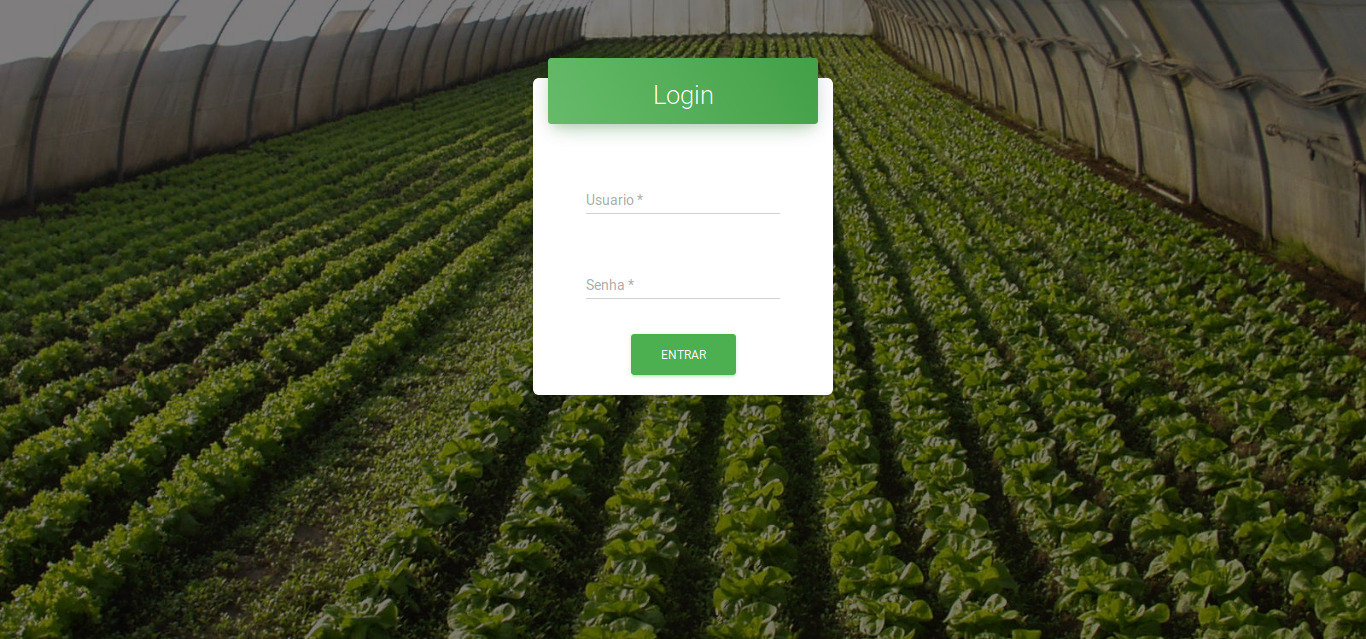
\includegraphics[scale=0.3]{04-figuras/tela_login.jpg}
    \caption{Tela de \textit{login} do sistema.}
    \vspace{-\baselineskip}
    \fonte{Do Autor (2018).}
    \label{fig:tela-login}
\end{figure}

\begin{figure}[H]
    \centering
    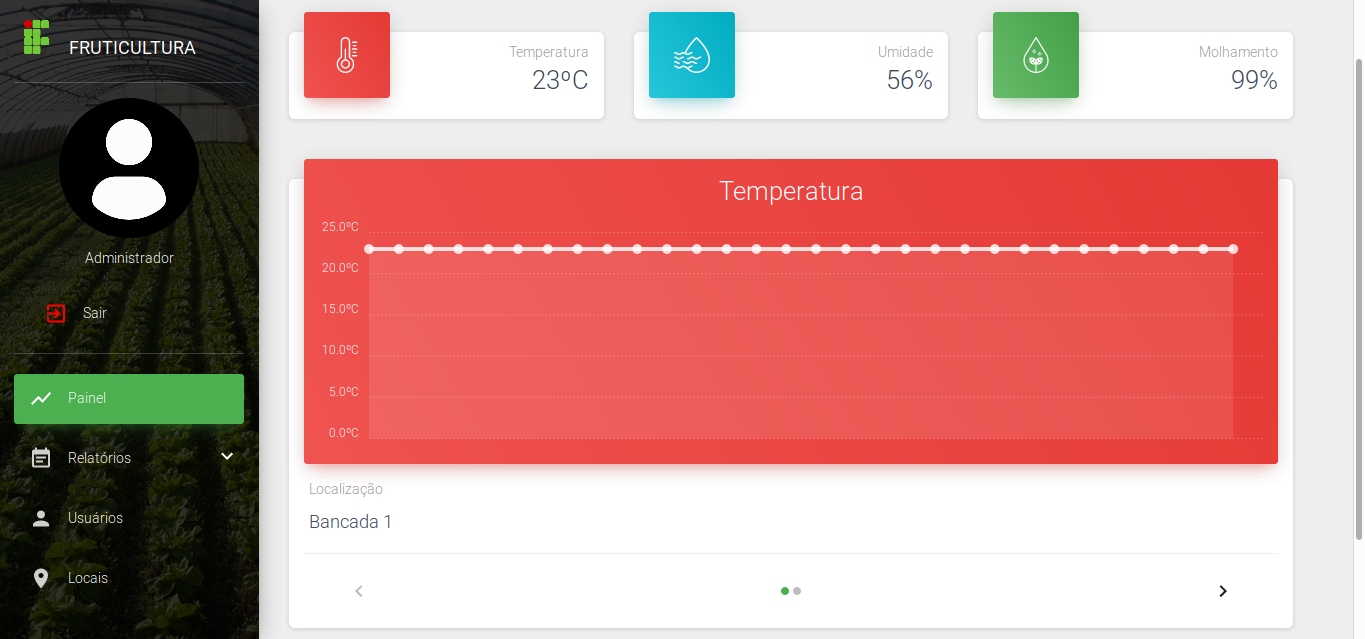
\includegraphics[scale=0.3]{04-figuras/tela_painel.png}
    \caption{Painel do sistema.}
    \vspace{-\baselineskip}
    \fonte{Do Autor (2018).}
    \label{fig:tela-dashboard}
\end{figure}

A figura \ref{fig:tela-listar-usuarios} mostra a tela onde é possível fazer a listagem dos usuários cadastrados no sistema, tendo também as ações de cadastrar ou excluir algum usuário listado. Já na figura \ref{fig:tela-cadastrar-usuario} temos o formulário utilizado para cadastrar um novo usuário e também atualizar as informações de um usuário já existente.

\begin{figure}[H]
    \centering
    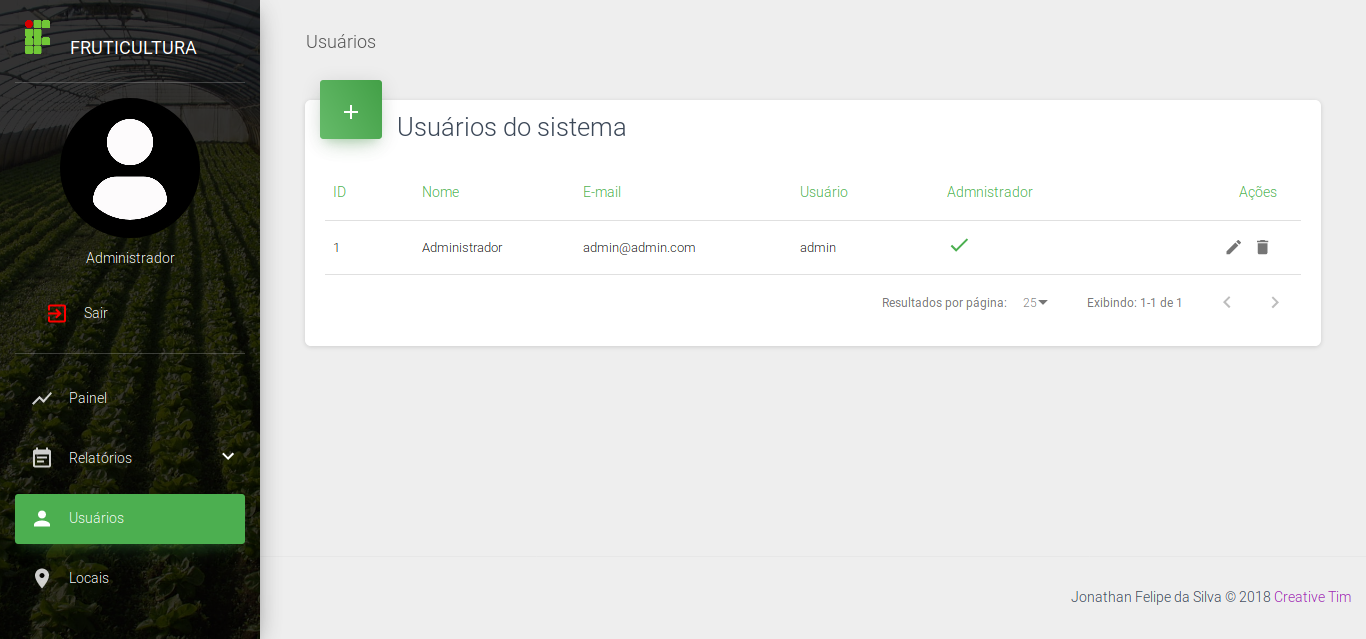
\includegraphics[scale=0.3]{04-figuras/tela_listar_usuarios.png}
    \caption{Tela de listar usuários.}
    \vspace{-\baselineskip}
    \fonte{Do Autor (2018).}
    \label{fig:tela-listar-usuarios}
\end{figure}

\begin{figure}[H]
    \centering
    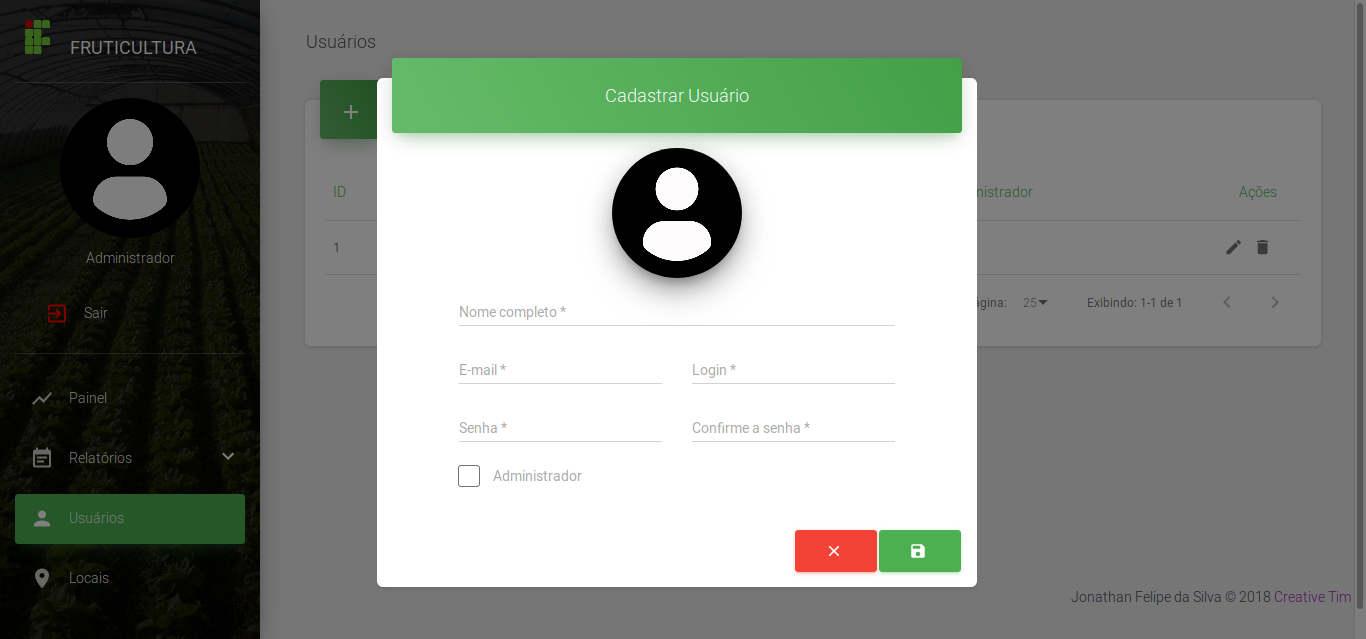
\includegraphics[scale=0.3]{04-figuras/tela_cadastrar_usuario.png}
    \caption{Tela de cadastrar novo usuário.}
    \vspace{-\baselineskip}
    \fonte{Do Autor (2018).}
    \label{fig:tela-cadastrar-usuario}
\end{figure}

A figura \ref{fig:tela-listar-locais} mostra a tela onde é possível fazer a listagem dos locais já cadastrados no sistema, tendo também as ações de cadastrar ou excluir algum local listado. Já na figura \ref{fig:tela-cadastrar-usuario} temos o formulário utilizado para cadastrar um novo local e também atualizar as informações de um local já cadastrado.

\begin{figure}[H]
    \centering
    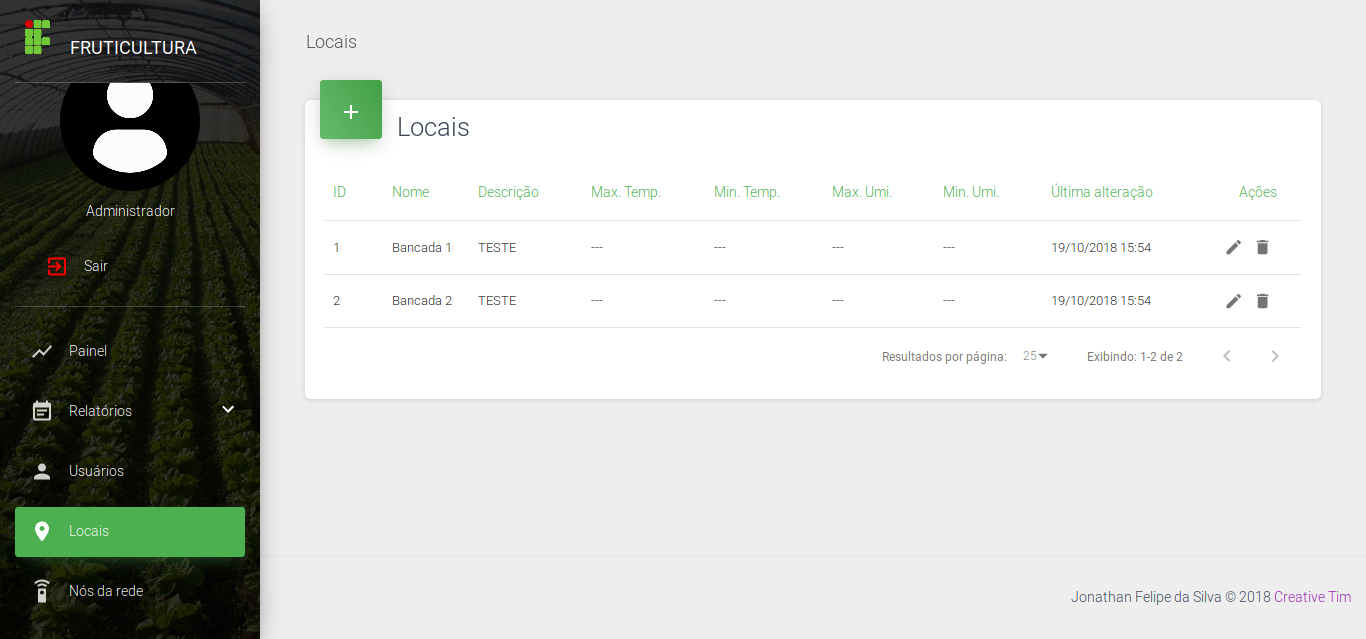
\includegraphics[scale=0.3]{04-figuras/tela_lista_locais.png}
    \caption{Tela de listar localizações dos nós.}
    \vspace{-\baselineskip}
    \fonte{Do Autor (2018).}
    \label{fig:tela-listar-locais}
\end{figure}

\begin{figure}[H]
    \centering
    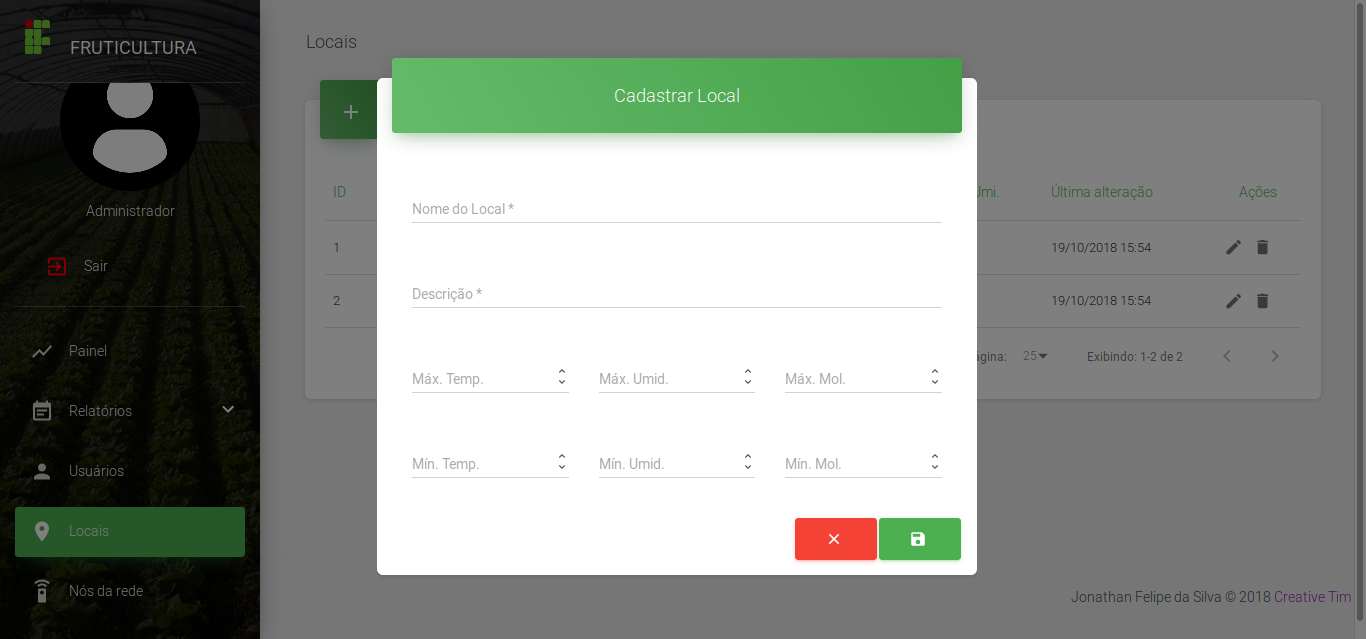
\includegraphics[scale=0.3]{04-figuras/tela_cadastra_local.png}
    \caption{Tela de cadastrar novo local.}
    \vspace{-\baselineskip}
    \fonte{Do Autor (2018).}
    \label{fig:tela-cadastrar-local}
\end{figure}

A figura \ref{fig:tela-listar-nos} mostra a tela onde é possível fazer a listagem dos nós já cadastrados no sistema, tendo também as ações de cadastrar ou excluir algum nó listado. Já na figura \ref{fig:tela-cadastrar-no} temos o formulário utilizado para cadastrar um novo nó e também atualizar as informações de um nó já cadastrado.

\begin{figure}[H]
    \centering
    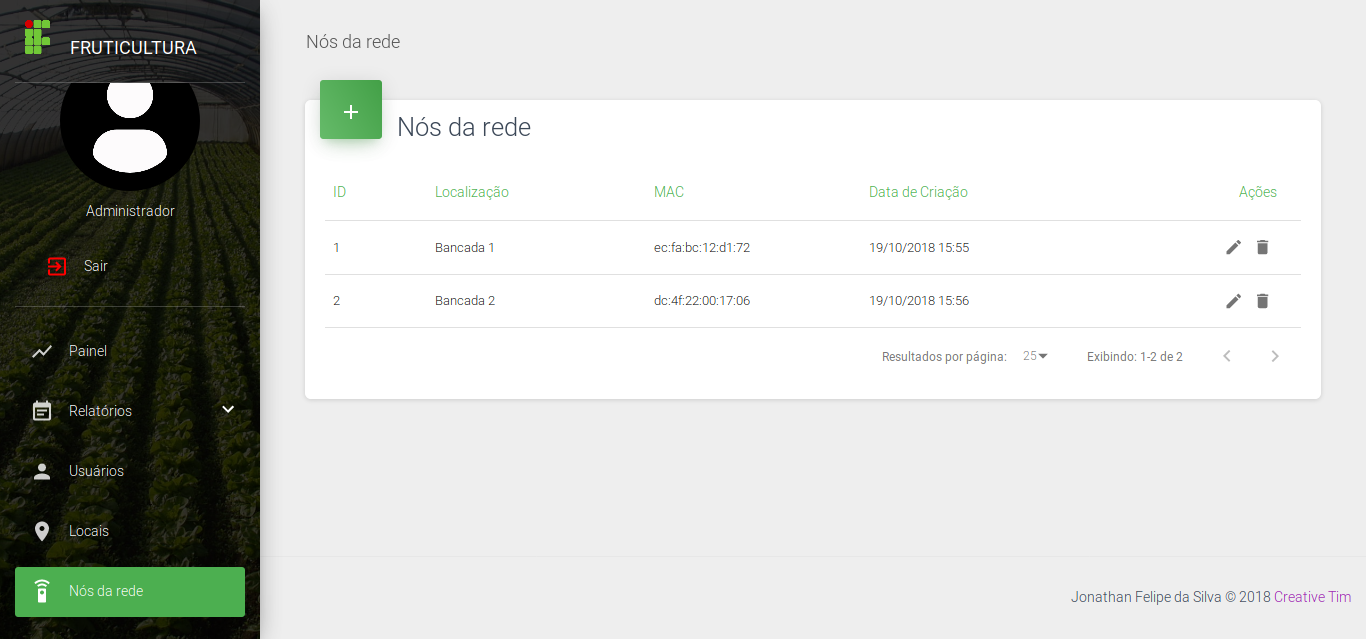
\includegraphics[scale=0.3]{04-figuras/tela_lista_no.png}
    \caption{Tela de listar nós da rede.}
    \vspace{-\baselineskip}
    \fonte{Do Autor (2018).}
    \label{fig:tela-listar-nos}
\end{figure}

\begin{figure}[H]
    \centering
    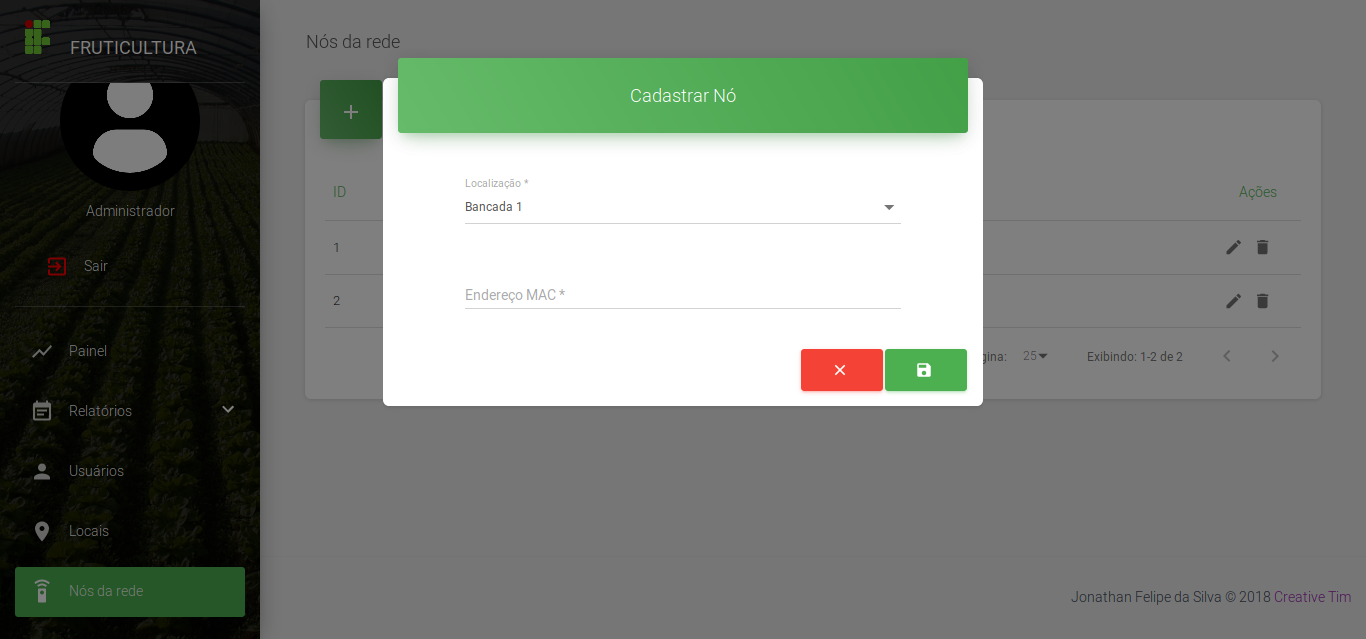
\includegraphics[scale=0.3]{04-figuras/tela_cadastra_no.png}
    \caption{Tela de cadastrar novo nó.}
    \vspace{-\baselineskip}
    \fonte{Do Autor (2018).}
    \label{fig:tela-cadastrar-no}
\end{figure}


A figura \ref{fig:tela-relatorio-medicoes} mostra a tela onde é emitir um relatório das medições realizadas pela rede em um determinado intervalo de tempo, além de também ter como ação visualizar todas as medições do dia. Já na figura \ref{fig:tela-relatorio-medicoes-dia} temos a listagem de todas as medições realizadas no dia em questão.

\begin{figure}[H]
    \centering
    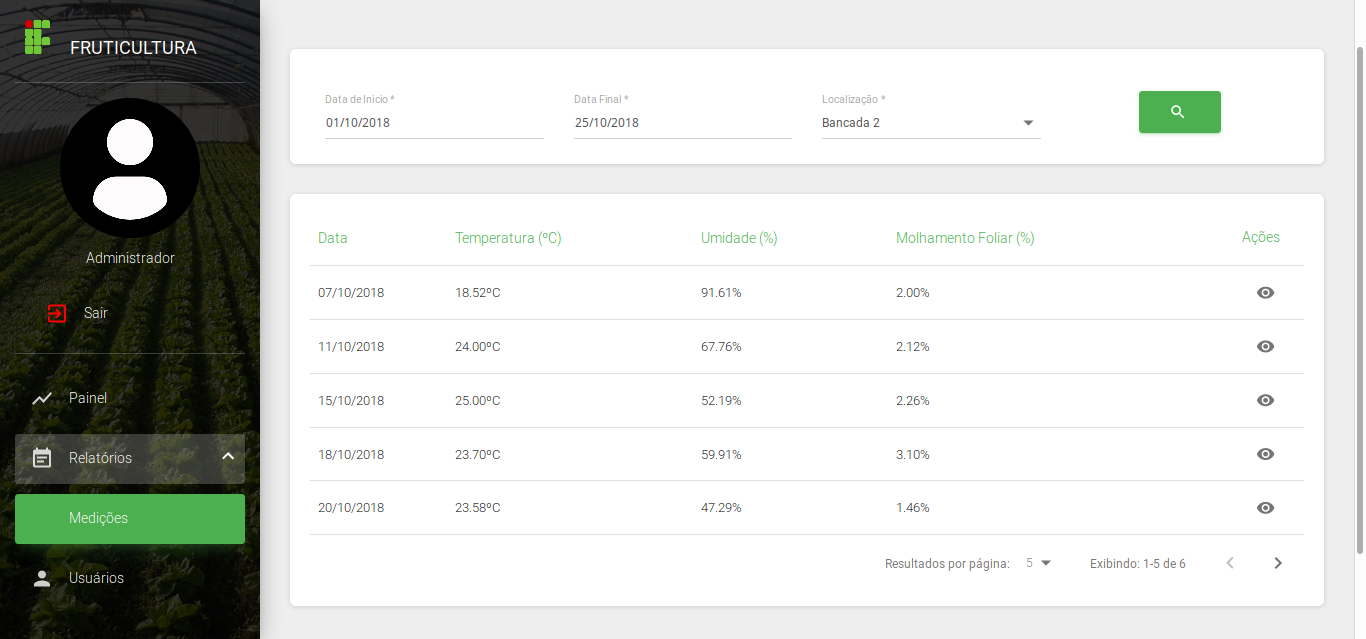
\includegraphics[scale=0.3]{04-figuras/tela_relatorio_medicoes.png}
    \caption{Tela de medições de um intervalo.}
    \vspace{-\baselineskip}
    \fonte{Do Autor (2018).}
    \label{fig:tela-relatorio-medicoes}
\end{figure}

\begin{figure}[H]
    \centering
    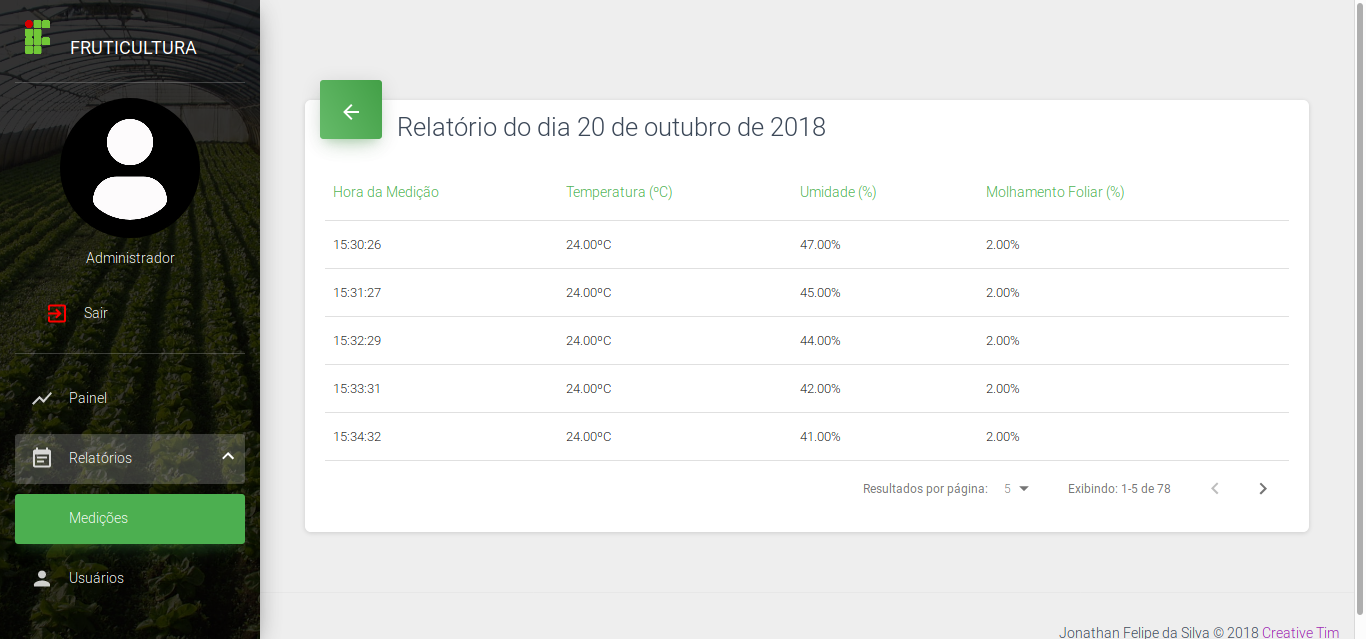
\includegraphics[scale=0.3]{04-figuras/tela_relatorio_medicoes_dia.png}
    \caption{Tela de medições de um dia.}
    \vspace{-\baselineskip}
    \fonte{Do Autor (2018).}
    \label{fig:tela-relatorio-medicoes-dia}
\end{figure}

Na Figura \ref{fig:relatorio-valvulas} é listado, a quantidade de vezes que o sistema nebulizador foi acionado no dia e a duração total em que o nebulizador ficou ativos, dentro de um intervalo informado. Além de ter também a opção de visualizar os acionamentos realizados em um dia específico. A Figura \ref{fig:relatorio-valvulas-detalhes} mostra apenas os acionamentos efetuado em um dia específicos.

\begin{figure}[H]
    \centering
    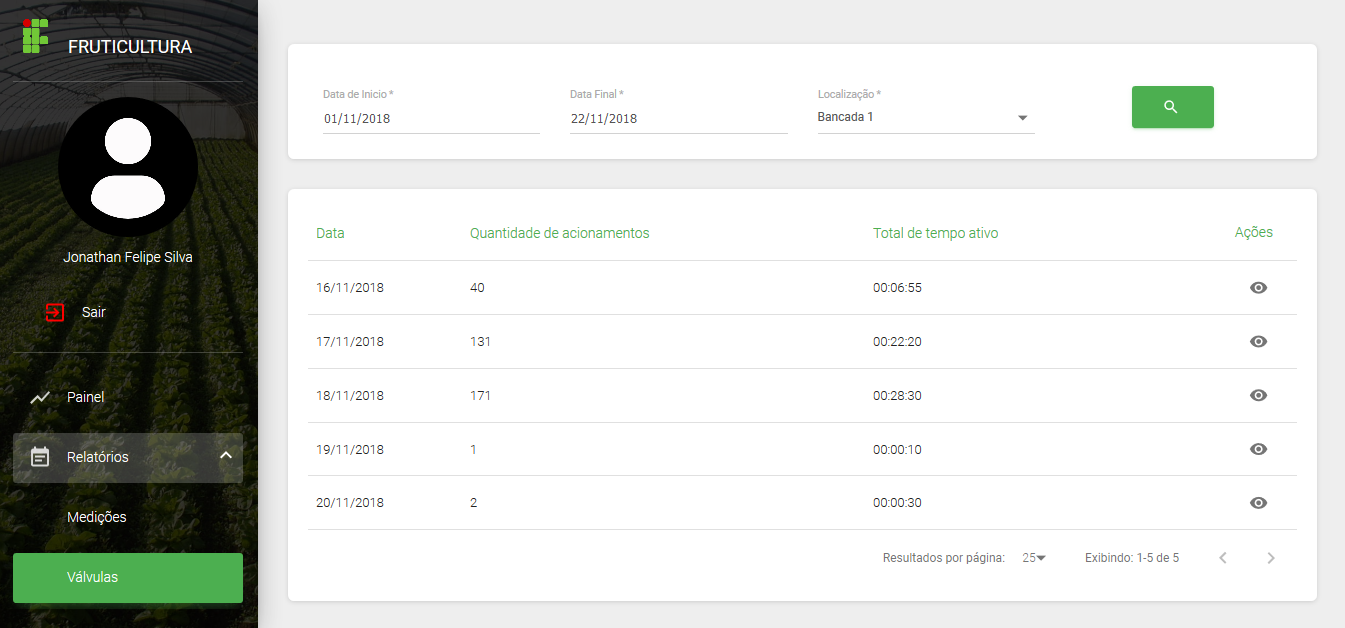
\includegraphics[scale=0.3]{04-figuras/relatorio-valvulas.png}
    \caption{Tela de acionamentos do nebulizador em um intervalo.}
    \vspace{-\baselineskip}
    \fonte{Do Autor (2018).}
    \label{fig:relatorio-valvulas}
\end{figure}

\begin{figure}[H]
    \centering
    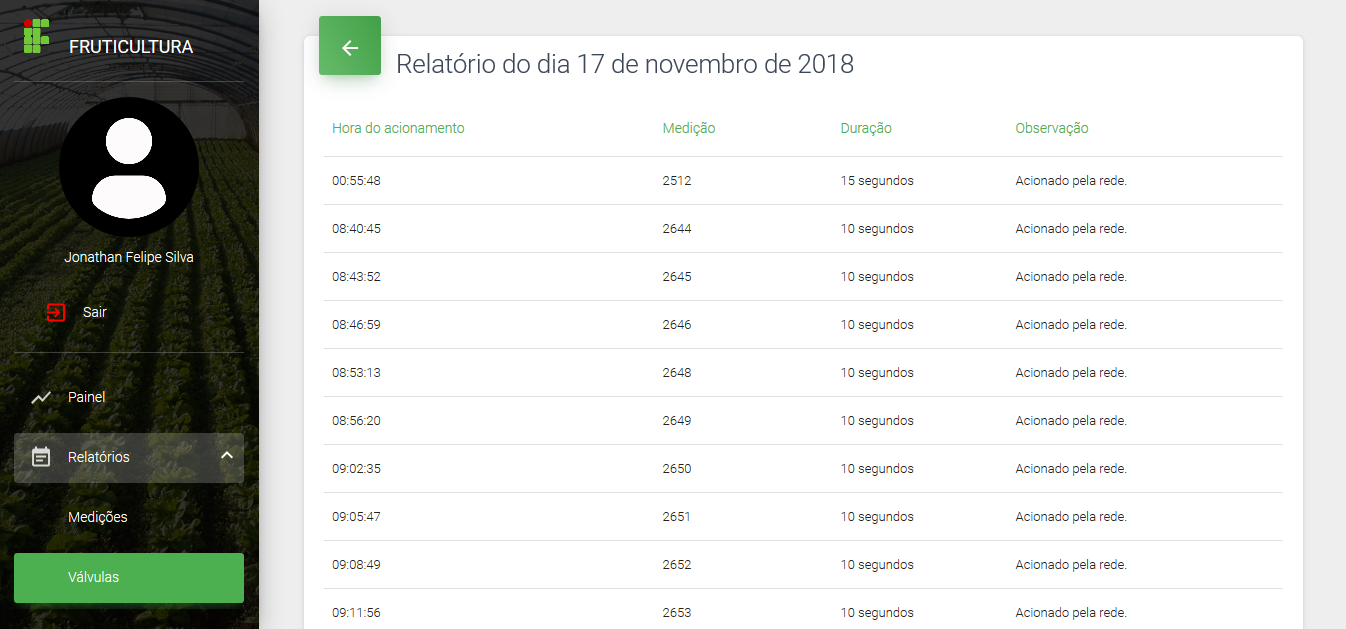
\includegraphics[scale=0.3]{04-figuras/relatorio-valvulas-detalhes.png}
    \caption{Tela de acionamentos do nebulizador em um dia.}
    \vspace{-\baselineskip}
    \fonte{Do Autor (2018).}
    \label{fig:relatorio-valvulas-detalhes}
\end{figure}

\subsection{Implantação do sistema}
Para se dar inicio aos testes do trabalho era necessário um servidor tanto para a aplicação web quanto para o \textit{broker} mqtt. Diante essa demanda foi criado uma conta na Amazon Web Services (AWS)\footnote[8]{Para maiores informações acesse: \url{https://aws.amazon.com/pt/}}, que é uma plataforma de serviços de computação em nuvem.

Com uma maquina virtual Linux disponibilizada pela AWS foi possível fazer a configuração de um servidor web com o Nginx\footnote[9]{Para maiores informações acesse: \url{https://www.nginx.com/}}
e também a configuração do \textit{broker} mqtt Mosquitto. Após concluir as configurações foi realizado o \textit{deploy} da aplicação, tanto backend quanto frontend, para o servidor\footnote[10]{A aplicação pode ser acessada em: \url{https://fruticultura.jonathanfsilva.me}}.

Com a aplicação em funcionamento, foi possível fazer a instalação dos nós dentro da estufa. A Figura \ref{fig:no-publicador-estufa} mostra um nó já instalado na estufa, fazendo a coleta dos valores de temperatura, umidade e molhamento foliar.

\begin{figure}[H]
    \centering
    \includegraphics[scale=0.1]{04-figuras/publicador-estufa.jpg}
    \caption{Nó publicador já instalado na estufa.}
    \vspace{-\baselineskip}
    \fonte{Do Autor (2018).}
    \label{fig:no-publicador-estufa}
\end{figure}
    \chapter{Considerações Finais}


% \section{Respondendo aos objetivos e contribuições do trabalho}


% \section{Proposta de Trabalhos Futuros}
    
    \postextual
    %
% Documento: Referências Bibliográficas
%

\bibliography{refbase}    % Geração automática das referências por meio do arquivo 'refbase.bib'

    % %
% Documento: Apêndices
%

\begin{apendicesenv}

% \chapter{Exemplo de Imagem}

% \begin{figure}[H]
%     \centering
%     \includegraphics[scale=0.5]{./04-figuras/navegar_abnt.png}
%     \caption{Exemplo de Imagem}
%     \label{fig:ilustfig}
% \end{figure}


\chapter{Exemplo de Tabela}

\begin{table}[H]
    \centering
    \caption[Exemplo tabela]{Exemplo tabela.\label{tab:exetab}}
    \begin{tabular}{|c|c|}
        \hline
            \textbf{Números x} & \textbf{Números y} \\
        \hline
             1 & 15     \\ \hline
             3 & 4      \\ \hline
             5 & 6      \\ \hline
             7 & 8      \\ \hline
			 9 & 11     \\ \hline
             13 & 15    \\
        \hline
    \end{tabular}
\end{table}

\end{apendicesenv}

    % %
% Documento: Anexos
%

\begin{anexosenv}

\chapter{Como elaborar}

Anexo é texto ou documento não elaborado pelo autor, que serve de fundamentação, comprovação e ilustração. Elemento opcional. Deve ser precedido da palavra ANEXO, identifi-cado por letras maiúsculas consecutivas, travessão e pelo respectivo título. Utilizam-se letras maiúsculas dobradas, na identificação dos anexos, quando esgotadas as letras do alfabeto.


\end{anexosenv}
    \printindex

\end{document}